\documentclass[11pt]{article}
\usepackage[a4paper,margin=1in]{geometry}
\usepackage[T1]{fontenc}
\usepackage[utf8]{inputenc}
\usepackage{amsmath,amssymb,amsthm,amsfonts,mathtools}
\usepackage{booktabs}
\usepackage{array}
\usepackage{adjustbox}
\usepackage{enumitem}
\usepackage{float}
\usepackage[table]{xcolor}
\usepackage{listings}
\usepackage{longtable}
\usepackage{tikz}
\usepackage{hyperref}
\usepackage{comment}
\usepackage[ruled,lined,linesnumbered]{algorithm2e}
\usetikzlibrary{arrows.meta,positioning}

\newtheorem{theorem}{Theorem}
\newtheorem{lemma}{Lemma}
\newtheorem{proposition}{Proposition}
\newtheorem{corollary}{Corollary}
\theoremstyle{definition}
\newtheorem{definition}{Definition}
\newtheorem{remark}{Remark}

\newcommand{\U}{\mathcal{U}_n}
\newcommand{\Ic}{I_c}
\newcommand{\J}{\mathcal{J}}
\newcommand{\Band}[2]{\mathcal{B}_{#1}^{#2}}
\newcommand{\Parity}[2]{\mathcal{P}_{#1}^{#2}}
\newcommand{\Weight}[2]{\mathcal{H}_{#1}^{#2}}
\newcommand{\bits}{\{0,1\}}
\definecolor{listinggray}{rgb}{0.5, 0.5, 0.5}
\definecolor{listinggrayer}{rgb}{0.95, 0.95, 0.95}
\lstdefinestyle{MathematicaStyle}{
    language=Mathematica,
    breaklines=true,
    breakatwhitespace=false,
    breakindent=1em,
    basicstyle=\ttfamily\scriptsize,
    columns=flexible,
    linewidth=0.9\linewidth,
    frame=single,
    showstringspaces=false,
    numbers=left,
    numberstyle=\tiny\color{listinggray},
    backgroundcolor=\color{listinggrayer},
    literate={+}{+}{1} {a}{a}{1} {b}{b}{1} {c}{c}{1} {d}{d}{1} {e}{e}{1} {f}{f}{1} {g}{g}{1} {h}{h}{1} {i}{i}{1} {j}{j}{1} {k}{k}{1} {l}{l}{1} {m}{m}{1} {n}{n}{1} {o}{o}{1} {p}{p}{1} {q}{q}{1} {r}{r}{1} {s}{s}{1} {t}{t}{1} {u}{u}{1} {v}{v}{1} {w}{w}{1} {x}{x}{1} {y}{y}{1} {z}{z}{1} {A}{A}{1} {B}{B}{1} {C}{C}{1} {D}{D}{1} {E}{E}{1} {F}{F}{1} {G}{G}{1} {H}{H}{1} {I}{I}{1} {J}{J}{1} {K}{K}{1} {L}{L}{1} {M}{M}{1} {N}{N}{1} {O}{O}{1} {P}{P}{1} {Q}{Q}{1} {R}{R}{1} {S}{S}{1} {T}{T}{1} {U}{U}{1} {V}{V}{1} {W}{W}{1} {X}{X}{1} {Y}{Y}{1} {Z}{Z}{1} {0}{0}{1} {1}{1}{1} {2}{2}{1} {3}{3}{1} {4}{4}{1} {5}{5}{1} {6}{6}{1} {7}{7}{1} {8}{8}{1} {9}{9}{1} {\}}{\}}{1},
    xleftmargin=1em,
    xrightmargin=1em
}

\title{Causal Index-Set Calculus for Boolean Networks and Deterministic Reconstruction}
\author{Alberto Hernández-Espinosa}
\date{}

\begin{document}
\maketitle

\begin{abstract}
We introduce a causality-first index-set calculus for Boolean networks in which the basic
object is not a sampled trajectory or a statistical summary, but the exact set of rules that
reconstructs network behaviour from local gate semantics over ordered exhaustive repertoires.
The calculus yields closed-form one-sets for monotone, parity, implication, threshold, and
canalising gate families; relates MSB-first and LSB-first enumerations by an explicit
bit-reversal involution; and reconstructs mixed-gate network outputs exactly by column-wise
composition of local index sets. Overlap among queried gate supports is exploited analytically
to compress the effective evaluation space from \(2^{d_q}\) to \(2^{\mu_q}\), where \(\mu_q\)
counts repeated coordinates. Deterministic benchmarks confirm exact equality to exhaustive
baselines at medium sizes (\(n\leq 13\)), exact sampled equality at larger sizes
(\(n\in\{20,50\}\)), and analytic evaluation of the order of a millisecond, independent of \(n\), at \(n=200\) under bounded
in-degree. The method provides a mathematically transparent alternative to brute-force
repertoire enumeration and to purely probabilistic surrogates when the generating mechanism
is known.
\end{abstract}

\section{Introduction}
Since classical mechanics, physics and the natural sciences have
treated causal structure, the identification of generative laws behind observed phenomena, as the
proper object of explanation, distinct from mere correlation or curve-fitting. Contemporary machine
learning and statistical AI, by contrast, largely approach causal structure indirectly: predictive models
are fit under strong distributional or parametric assumptions, and causal claims are recovered only
approximately, conditional on those assumptions holding. Judea Pearl's causal calculus formalised this gap
within statistics itself, showing that interventionist causal claims require machinery beyond
observational correlation \cite{pearl2009causality}.

On the other hand, algorithmic probability, rooted in the foundational work of Solomonoff,
Kolmogorov, and Chaitin \cite{solomonoff1964formal,kolmogorov1965three,chaitin1966length}, and
developed as algorithmic information dynamics \cite{zenilcalculus,zenildeconv}, is closely aligned
with the Principle of Computational Equivalence (PCE) \cite{wolfram2002new}, which holds that short
generative rules are, in principle, responsible for the full complexity observed in natural and
computational systems. While PCE is a thesis about the world, the algorithmic-causality framework
is an inferential and interventionist calculus for recovering such rules from observations
\cite{zenilcalculus}. The present work aims at a concrete materialisation of the same underlying
idea: it uses Boolean networks as an explicit artefact in which small local rules are shown,
deterministically and in closed form, to generate the full complexity of the network's behaviour.

The central difficulty in Boolean-network analysis is therefore not lack of computational power; it is
lack of causal compression. One can always enumerate a repertoire, print a truth table, or run a
simulation. What remains elusive is a representation that is at once exact, compositional, and
explanatory. For a high-level scientific treatment, this distinction matters: a method that merely
reproduces outputs is weaker than a method that identifies the rule structure responsible for them.

This paper advances the following thesis. Ordered exhaustive repertoires contain a non-trivial algebraic
structure, and this structure can be exploited to replace brute-force enumeration by exact causal formulae.
Once the ordering convention is fixed, the question ``what can this network do?'' can be recast as ``at
which conditions is each local rule active, and how do those conditions compose?'' The result is an
index-set calculus for Boolean networks.

A terminological clarification is needed at the outset. The word ``causal'' is used in this paper
in the \emph{mechanistic} or \emph{generative} sense: the Boolean network is the causal mechanism,
and the index-set formula reconstructs the exact input--output map of that mechanism. This usage
follows the tradition of mechanistic explanation in philosophy of science
\cite{machamer2000thinking,woodward2003making} and of generative modelling in algorithmic
information theory \cite{zenilcalculus}, rather than the interventionist \emph{do}-calculus of
Pearl \cite{pearl2009causality}. The present calculus does not perform causal discovery from
observational data, nor does it reason about interventions or confounders. It derives the exact
consequences of a \emph{known} generative rule. Where Pearl's framework asks ``what would happen
if we intervened on variable \(X\)?'', the present framework asks ``at which repertoire positions
does the known rule for node \(i\) produce output one, and how do these positions compose across
the network?''

The perspective is causality-first in three senses. First, it is rule-first rather than correlation-first:
the object of study is the generative logic of the system, not only its observed frequencies, the same
distinction that separates physical law from statistical regression. Second, it is deterministic rather
than statistical: the method aims at exact reconstruction under known dynamics, not at approximate
inference under unknown mechanisms, departing from the assumption-laden regime of modern statistical
learning. Third, it is compositional: global behaviour is built from local causal rules rather than from
opaque end-to-end approximations.

This perspective connects two traditions. The first is PCE \cite{wolfram2002new}, which
demonstrates that simple discrete rules generate the full complexity observed in natural and
computational systems. The second is the algorithmic-causality programme
\cite{zenilcalculus,zenildeconv}, which treats complex systems as computational objects and
provides an intervention-oriented calculus for discovering and steering hidden generating
mechanisms from observations, emphasising algorithmic probability, generative mechanisms, and
causation over surface statistics.

While the present contribution is inspired by both traditions, its objective is distinct. We
assume the local Boolean rules and network structure are given, and we derive exact mathematical
expressions for the resulting behaviour over the full ordered repertoire. In that sense, the method is less
a causal-discovery calculus than a causal-expression calculus. It remains connected to algorithmic
probability and to the idea that simple rules can underwrite rich behaviour, but it is more law-like in the
narrow physical sense: the target is a closed-form deterministic description of behaviour, not an
approximate recovery of an unknown generator. This is precisely why the work is also close in spirit to
Wolfram's emphasis on exact discrete rules \cite{wolfram2002new}, while differing from purely statistical
or machine-learning approaches that learn predictive regularities without recovering the underlying
analytic form \cite{pearl2009causality}.


In what follows, we show that ordered exhaustive repertoires admit an algebraic structure that supports exact, network-aware one-set formulae for all canonical gate families; that ordering changes are controlled by an explicit involution, rendering exactness invariant under representation; and that mixed-gate synchronous networks can be reconstructed exactly by composing local index sets. The resulting complexity improvements arise not by removing the \(2^n\) state space but by replacing brute-force gate evaluation with explicit causal formulae, enabling exact query answering without full matrix materialisation, and reducing the validation burden through principled sampling.

Sections~2 and~3 define the ordered-repertoire formalism and the index objects needed for exact reasoning. Section~4 derives the gate-family one-sets and their expanded forms, and presents worked examples including a detailed AND deconvolution, a composed XOR case, and a 10-node mixed-gate benchmark with overlap analysis and dynamical enrichment. Section~5 proves ordering invariance, and Section~6 characterises the scalability and resource envelope of exact causal evaluation together with a validation summary. The appendices collect exact gate expansions, sensitivity formulae, the validation artefact index, and an extended experimental programme. All computational experiments are reproducible via the companion code repository (see Appendix~C for details).

\section{Formal Setup}
Let \(cm \in \bits^{n \times n}\) be the connectivity matrix of a Boolean network, where \(cm_{ij}=1\) means that node \(j\) feeds node \(i\). Let
\[
dynamic=(d_1,\dots,d_n)
\]
be the list of local gate labels, and let
\[
N_i=\{j\in\{1,\dots,n\} : cm_{ij}=1\}
\]
be the connected-input set of node \(i\). Each node has a local map
\[
g_i:\bits^{|N_i|}\to\bits,
\]
and the synchronous one-step network update is
\[
F(x)=\bigl(g_1(x_{N_1}),\dots,g_n(x_{N_n})\bigr), \qquad x\in\bits^n.
\]

\begin{definition}[Ordered Exhaustive Repertoire]
The ordered exhaustive repertoire of size \(n\) is the set \(\bits^n\) together with a declared enumeration of all \(2^n\) binary vectors. We write \(\U=\{1,\dots,2^n\}\) for the corresponding index universe.
\end{definition}

Two orderings are operationally relevant throughout the project.
\begin{itemize}
\item \textbf{LSB-first ordering:} the index \(j\) is associated with \(v(j)=\mathrm{Reverse}(\mathrm{IntegerDigits}(j-1,2,n))\), with weights \(2^{i-1}\).
\item \textbf{MSB-first ordering:} the index \(j\) is associated with \(v(j)=\mathrm{IntegerDigits}(j-1,2,n)\), with weights \(2^{n-i}\).
\end{itemize}

\begin{definition}[Bit-Reversal Involution]
For \(j\in\U\), define
\[
\varphi(j)=1+\mathrm{FromDigits}\Bigl(\mathrm{Reverse}\bigl(\mathrm{IntegerDigits}(j-1,2,n)\bigr),2\Bigr).
\]
Then \(\varphi:\U\to\U\) is an involution.
\end{definition}

The involution \(\varphi\) is not a cosmetic convenience. It is the formal device that makes ordering control explicit. Without it, one risks confusing genuine mathematical differences with mere encoding differences.

\section{Causal Index Sets}
The method begins with a structural observation: each coordinate of an ordered exhaustive repertoire forms periodic bands, and Boolean gates can be expressed as exact set operations on those bands.

\begin{definition}[Bit Bands]
For a node index \(i\in\{1,\dots,n\}\) and a bit value \(a\in\bits\), define
\[
\Band{i}{a}=\{j\in\U : v_i(j)=a\}.
\]
\end{definition}

\begin{definition}[Parity and Weight Classes]
For a connected-input set \(\Ic\subseteq\{1,\dots,n\}\), define
\[
\Parity{\Ic}{1}=\Bigl\{j\in\U : \sum_{i\in\Ic} v_i(j)\equiv 1 \pmod 2 \Bigr\},
\]
\[
\Parity{\Ic}{0}=\Bigl\{j\in\U : \sum_{i\in\Ic} v_i(j)\equiv 0 \pmod 2 \Bigr\},
\]
and for \(r\in\{0,\dots,|\Ic|\}\),
\[
\Weight{\Ic}{r}=\Bigl\{j\in\U : \sum_{i\in\Ic} v_i(j)=r \Bigr\}.
\]
\end{definition}

\begin{definition}[Decimal Weights, Anchors, and Sumandos]
Let the ordering policy be fixed. Define the bit weight
\[
w(i)=
\begin{cases}
2^{i-1}, & \text{LSB-first},\\
2^{n-i}, & \text{MSB-first}.
\end{cases}
\]
For \(S\subseteq\{1,\dots,n\}\) and \(\eta\in\bits^{|S|}\), define the offset
\[
\Delta_S(\eta)=\sum_{t\in S}\eta_t\,w(t),
\]
and for a connected-input set \(\Ic\), define the AND decimal anchor
\[
P(\Ic)=\sum_{i\in\Ic} w(i).
\]
\end{definition}

These three families already encode most of the method. Bands capture fixed-bit conditions,
parity classes capture XOR-like structure, and Hamming-weight strata capture threshold logic.
The following sections show that standard gate families are simple set expressions built from them.

\begin{definition}[Deconvolution Operator]
For finite sets \(L,S\subset\mathbb{Z}\), define
\[
\operatorname{Dec}(L,S)=\{\ell+s:\ell\in L,\ s\in S\}.
\]
This operator unfolds a compressed pair \((L,S)\) into the full set of repertoire indices.
When \(L\) is a base set of decimal anchors and \(S\) is the offset family generated by the
free coordinates, \(\operatorname{Dec}(L,S)\) recovers the exact one-set without row-wise
gate evaluation.
\end{definition}

\begin{remark}[Terminology: Deconvolution versus Minkowski Sum]
The set-addition form \(\{\ell+s:\ell\in L,\,s\in S\}\) resembles the Minkowski sum of two
point sets in \(\mathbb{Z}\). The term \emph{deconvolution} is used here advisedly, because the
operation reverses the combinatorial convolution that produces a composite repertoire index from
independent subsystem contributions: the base set \(L\) encodes the constrained (connected)
coordinates, the offset set \(S\) encodes the free (disconnected) coordinates, and
\(\operatorname{Dec}\) reconstructs the full index set from these two factors. In signal-processing
terms, the composite index is the ``convolved'' signal and \(\operatorname{Dec}\) recovers the
constituent structure. The distinction from a generic Minkowski sum is that the two factors here
have a definite causal interpretation (constrained versus free coordinates) rather than being
arbitrary point sets in a metric space.
\end{remark}

\section{Exact Gate Formulae}
The following proposition collects the exact one-set formulae for the gate families supported by the calculus.

\begin{proposition}[Gate-Family One-Sets]\label{prop:gate-family-one-sets}
Let node \(k\) have connected-input set \(\Ic\). Under a fixed repertoire ordering, the set of indices at which node \(k\) outputs one is given as follows.
\begin{center}
\small
\begin{tabular}{p{0.20\linewidth}p{0.67\linewidth}}
\toprule
\textbf{Gate family} & \textbf{Exact one-set formula} \\
\midrule
AND & \(\J_k^{\mathrm{AND}}=\bigcap_{i\in\Ic}\Band{i}{1}\) \\
OR & \(\J_k^{\mathrm{OR}}=\bigcup_{i\in\Ic}\Band{i}{1}\) \\
NAND & \(\J_k^{\mathrm{NAND}}=\U\setminus \J_k^{\mathrm{AND}}\) \\
NOR & \(\J_k^{\mathrm{NOR}}=\bigcap_{i\in\Ic}\Band{i}{0}=\U\setminus \J_k^{\mathrm{OR}}\) \\
XOR & \(\J_k^{\mathrm{XOR}}=\Parity{\Ic}{1}\) \\
XNOR & \(\J_k^{\mathrm{XNOR}}=\Parity{\Ic}{0}\) \\
NOT on input \(r\) & \(\J_k^{\mathrm{NOT}}=\Band{r}{0}\) \\
IMPLIES on pair \((a,b)\) & \(\J_k^{\mathrm{IMP}}=\Band{a}{0}\cup\bigl(\Band{a}{1}\cap\Band{b}{1}\bigr)\), equivalently \(\U\setminus\bigl(\Band{a}{1}\cap\Band{b}{0}\bigr)\) \\
NIMPLIES on pair \((a,b)\) & \(\J_k^{\mathrm{NIMP}}=\Band{a}{1}\cap\Band{b}{0}\) \\
KOFN threshold & \(\J_k^{\mathrm{KOFN}}=\bigcup_{r=k}^{|\Ic|}\Weight{\Ic}{r}\) \\
Strict-EXACT-\(k\) & \(\J_k^{=k}=\Weight{\Ic}{k}\) \\
Canalising with trigger set \(C\), trigger output \(o\), and fallback one-set \(\J_h\) & \(\J_k^{\mathrm{CAN}}=C\cup\bigl((\U\setminus C)\cap \J_h\bigr)\) if \(o=1\); \(\J_k^{\mathrm{CAN}}=(\U\setminus C)\cap \J_h\) if \(o=0\) \\
\bottomrule
\end{tabular}
\end{center}
\end{proposition}

\begin{proof}
We verify each gate family by establishing a bijection between its standard Boolean semantics and the stated set expression.

\emph{AND/OR.} By definition, \(g^{\mathrm{AND}}(x_{N_k})=1\) if and only if \(x_i=1\) for every \(i\in\Ic\). The set of indices satisfying this condition is exactly \(\bigcap_{i\in\Ic}\Band{i}{1}\). The OR case follows by duality: \(g^{\mathrm{OR}}=1\) iff at least one connected input equals one, which is \(\bigcup_{i\in\Ic}\Band{i}{1}\).

\emph{NAND/NOR.} These are complements: \(\J^{\mathrm{NAND}}=\U\setminus\J^{\mathrm{AND}}\) and \(\J^{\mathrm{NOR}}=\U\setminus\J^{\mathrm{OR}}=\bigcap_{i\in\Ic}\Band{i}{0}\), since requiring all connected inputs to be zero is equivalent to excluding every one-band.

\emph{XOR/XNOR.} The XOR output equals one exactly when the number of active connected inputs is odd: \(\sum_{i\in\Ic}v_i(j)\equiv 1\pmod{2}\), which is the definition of \(\Parity{\Ic}{1}\). XNOR is the complementary parity class.

\emph{NOT.} With a single designated input \(r\), the output is one exactly when \(v_r(j)=0\), giving \(\Band{r}{0}\).

\emph{IMPLIES/NIMPLIES.} For the ordered pair \((a,b)\), non-implication \(a\wedge\neg b\) holds exactly on \(\Band{a}{1}\cap\Band{b}{0}\). Implication is the complement of this set in \(\U\).

\emph{KOFN/exact-\(k\).} The output equals one when \(\sum_{i\in\Ic}v_i(j)\geq k\), i.e.\ when the Hamming weight on the connected inputs lies in layers \(\{k,k+1,\ldots,|\Ic|\}\). This is \(\bigcup_{r=k}^{|\Ic|}\Weight{\Ic}{r}\). The exact-\(k\) variant restricts to the single layer \(\Weight{\Ic}{k}\).

\emph{Canalising.} Let the trigger set be \(C\). When the canalising input takes its trigger value, the output is forced to \(o\). On the complement \(\U\setminus C\), the output follows the fallback rule with one-set \(\J_h\). If \(o=1\), the full one-set is \(C\cup((\U\setminus C)\cap\J_h)\); if \(o=0\), the trigger band forces zero, so the one-set is \((\U\setminus C)\cap\J_h\).
\end{proof}

\begin{remark}
The decisive point is that these are \emph{network-aware} formulae. The local rule is not written abstractly over unnamed inputs; it is anchored to the actual connected-input set \(\Ic\) induced by the network topology.
\end{remark}

\subsection{Expanded Gate Expressions}
This section introduces the explicit derived expressions 
for each of the supported gates for the calculation.

\paragraph{AND.}
Let \(I_{nc}=\{1,\dots,n\}\setminus \Ic\). The connected bits are fixed to one, so the decimal contribution of the connected part is the decimal anchor
\[
P(\Ic)=\sum_{i\in\Ic} w(i).
\]
The disconnected bits provide the free offset
\[
\Delta_{nc}(\eta)=\sum_{t\in I_{nc}} \eta_t\,w(t), \qquad \eta\in\bits^{|I_{nc}|}.
\]
Hence the one-set can be written as
\[
\J_k^{\mathrm{AND}}
=
\Bigl\{\,1+P(\Ic)+\Delta_{nc}(\eta)\ \Big|\ \eta\in\bits^{|I_{nc}|}\Bigr\},
\]
equivalently
\[
\J_k^{\mathrm{AND}}=\{j\in\U:\forall i\in\Ic,\ v_i(j)=1\}.
\]

\paragraph{OR.}
For each connected input \(i\in\Ic\), define the one-band
\[
\mathcal{B}_i^{(1)}
=
\Bigl\{\,1+w(i)+\Delta_{\{1,\dots,n\}\setminus\{i\}}(\eta)\ \Big|\
\eta\in\bits^{n-1}\Bigr\}.
\]
Then
\[
\J_k^{\mathrm{OR}}=\bigcup_{i\in\Ic}\mathcal{B}_i^{(1)}
=
\{j\in\U:\exists i\in\Ic,\ v_i(j)=1\}.
\]

\paragraph{NAND.}
The zero-set of NAND is exactly the one-set of AND, so
\[
\mathcal{Z}_k^{\mathrm{NAND}}
=
\J_k^{\mathrm{AND}}
=
\Bigl\{\,1+P(\Ic)+\Delta_{nc}(\eta)\ \Big|\ \eta\in\bits^{|I_{nc}|}\Bigr\},
\]
and the one-set is its complement:
\[
\J_k^{\mathrm{NAND}}=\U\setminus \mathcal{Z}_k^{\mathrm{NAND}}.
\]

\paragraph{NOR.}
For each \(i\in\Ic\), define the zero-band
\[
\mathcal{B}_i^{(0)}
=
\Bigl\{\,1+\Delta_{\{1,\dots,n\}\setminus\{i\}}(\eta)\ \Big|\
\eta\in\bits^{n-1}\Bigr\},
\]
which enforces \(v_i=0\). Then
\[
\J_k^{\mathrm{NOR}}=\bigcap_{i\in\Ic}\mathcal{B}_i^{(0)}
=
\{j\in\U:\forall i\in\Ic,\ v_i(j)=0\}
=
\U\setminus\J_k^{\mathrm{OR}}.
\]

\paragraph{XOR and XNOR.}
These families are controlled by the parity of the connected bits:
\[
\J_k^{\mathrm{XOR}}
=
\Bigl\{\,j\in\U\ \Big|\
\sum_{i\in\Ic}v_i(j)\equiv 1\pmod 2
\Bigr\},
\]
\[
\J_k^{\mathrm{XNOR}}
=
\Bigl\{\,j\in\U\ \Big|\
\sum_{i\in\Ic}v_i(j)\equiv 0\pmod 2
\Bigr\}
=
\U\setminus\J_k^{\mathrm{XOR}}.
\]
No decimal-anchor-plus-sumandos decomposition is needed here because the relevant invariant is parity rather than a single threshold band.

\paragraph{NOT.}
For a designated input index \(r\), the NOT one-set is the zero-band of that input:
\[
\J_k^{\mathrm{NOT}}=\Band{r}{0}
=
\Bigl\{\,1+\Delta_{\{1,\dots,n\}\setminus\{r\}}(\eta)\ \Big|\
\eta\in\bits^{n-1}\Bigr\}.
\]

\paragraph{IMPLIES and NIMPLIES.}
For an ordered pair \((a,b)\), the forbidden asymmetric pattern is \(a=1,b=0\). Its index set is
\[
\mathcal{B}_{a=1,b=0}
=
\Bigl\{\,1+w(a)+\Delta_{\{1,\dots,n\}\setminus\{a,b\}}(\eta)\ \Big|\
\eta\in\bits^{n-2}\Bigr\}.
\]
Therefore
\[
\J_k^{\mathrm{NIMP}}=\mathcal{B}_{a=1,b=0},
\qquad
\J_k^{\mathrm{IMP}}=\U\setminus\mathcal{B}_{a=1,b=0}.
\]
Equivalently,
\[
\J_k^{\mathrm{IMP}}=\{j\in\U:\neg v_a(j)\ \lor\ v_b(j)\},
\qquad
\J_k^{\mathrm{NIMP}}=\{j\in\U:v_a(j)=1,\ v_b(j)=0\}.
\]

\paragraph{KOFN threshold family.}
For threshold \(k\),
\[
\J_k^{\mathrm{KOFN}}
=
\bigcup_{r=k}^{|\Ic|}\Weight{\Ic}{r}
=
\Bigl\{\,j\in\U\ \Big|\
\sum_{i\in\Ic} v_i(j)\ge k
\Bigr\}.
\]
For strict-exact thresholding,
\[
\J_k^{=k}=\Weight{\Ic}{k}
=
\Bigl\{\,j\in\U\ \Big|\
\sum_{i\in\Ic} v_i(j)=k
\Bigr\}.
\]
Thus threshold families are controlled by Hamming-weight layers rather than by parity or a single decimal anchor. The MAJORITY gate is the special case \(k=\lceil|\Ic|/2\rceil\), so its one-set is the union of weight layers at or above the strict majority threshold.

\paragraph{Canalising family.}
Let the canalising input be \(c\), the canalising value be \(\nu\in\bits\), the trigger output be \(o\in\bits\), and the fallback one-set be \(\J_h\). Define the trigger set
\[
C_{c,\nu}=\{j\in\U:v_c(j)=\nu\}.
\]
Then the one-set is
\[
\J_k^{\mathrm{CAN}}
=
\begin{cases}
C_{c,\nu}\cup\bigl((\U\setminus C_{c,\nu})\cap \J_h\bigr), & o=1,\\[4pt]
(\U\setminus C_{c,\nu})\cap \J_h, & o=0.
\end{cases}
\]
In the current implementation the fallback rule is OR on the remaining inputs, so \(\J_h\) is typically an OR-type union of one-bands outside the trigger case.

\subsection{Dynamic Properties and Pattern Taxonomy}
The exact one-set calculus is not only a static indexing device. It also recovers dynamic properties
of the system: monotonicity class, average sensitivity under the uniform exhaustive repertoire, and the coarse pattern symbol induced by a node's full output column.

\begin{definition}[Column-Wise Pattern Symbol]
Let \(Y\in\bits^{2^n\times n}\) be the output matrix over the ordered exhaustive repertoire. For node \(i\), define
\[
\pi_i=
\begin{cases}
0, & \text{if } \sum_{j=1}^{2^n} Y_{j,i}=0,\\
1, & \text{if } \sum_{j=1}^{2^n} Y_{j,i}=2^n,\\
*, & \text{otherwise.}
\end{cases}
\]
\end{definition}

This three-symbol alphabet captures a useful distinction that repeatedly appears in the validation programme. Some rules are structurally non-trivial but still constant over a declared repertoire because parameters collapse them to extreme cases; others remain genuinely varying and therefore receive the symbol \(*\).

\begin{proposition}[Dynamic Summary of Canonical Gate Families]\label{prop:dynamic-summary}
For a gate of arity \(d\) under the uniform exhaustive repertoire, the families in Table~\ref{tab:dynamic-pattern-summary} satisfy the listed monotonicity, average sensitivity, and pattern behaviour.
\end{proposition}

\begin{table}[t]
\centering
\small
\begin{tabular}{p{0.17\linewidth}p{0.18\linewidth}p{0.24\linewidth}p{0.28\linewidth}}
\toprule
\textbf{Family} & \textbf{Monotonicity} & \textbf{Average sensitivity} & \textbf{Pattern over exhaustive inputs} \\
\midrule
AND / OR & monotone increasing & \(\bar{s}=d/2^{d-1}\) & \(*\) except degenerate unary or fixed-input cases \\
NAND / NOR & monotone decreasing & \(\bar{s}=d/2^{d-1}\) & \(*\) except degenerate unary or fixed-input cases \\
XOR / XNOR & parity-based, non-monotone & \(\bar{s}=d\) & always \(*\) for non-empty connected-input sets \\
NOT & anti-monotone & \(\bar{s}=1\) & \(*\) \\
IMPLIES / NIMPLIES & asymmetric, mixed monotonicity in ordered pair & \(\bar{s}=1\) for the binary case & typically \(*\) \\
KOFN & monotone increasing & \(\bar{s}=d\binom{d-1}{k-1}/2^{d-1}\) & \(1\) if \(k=0\), \(0\) if \(k>d\), otherwise \(*\) \\
strict-KOFN & monotone increasing & \(\bar{s}=d\binom{d-1}{k}/2^{d-1}\) & \(1\) if \(k<0\), \(0\) if \(k\ge d\), otherwise \(*\) \\
CANALISING & depends on fallback rule, but collapses on trigger band & reduced on trigger band; exact value depends on fallback & constant on trigger band; globally \(0\), \(1\), or \(*\) depending on fallback and trigger output \\
\bottomrule
\end{tabular}
\caption{Dynamic properties of the exact gate families: monotonicity class, average sensitivity under the uniform exhaustive repertoire, and the resulting coarse pattern symbol \(\pi_i\).}
\label{tab:dynamic-pattern-summary}
\end{table}

\begin{proof}
Average sensitivity \(\bar{s}\) counts, for each input position, the fraction of input vectors on which flipping that position changes the output, then sums over all positions.

\emph{AND/OR.} For AND of arity \(d\), flipping input \(i\) changes the output only when all other inputs equal one. There are \(2^{d-1}\) total assignments to the remaining inputs, and exactly one of them (all ones) is sensitive. Summing over all \(d\) inputs gives \(\bar{s}=d/2^{d-1}\). By De Morgan duality, OR has the same average sensitivity.

\emph{XOR/XNOR.} Flipping any single input toggles the parity of the sum. Therefore every input is sensitive on every input vector, giving \(\bar{s}=d\).

\emph{NOT.} The single input is always sensitive: \(\bar{s}=1\).

\emph{KOFN.} Flipping input \(i\) changes the output if and only if the remaining \(d-1\) inputs have Hamming weight exactly \(k-1\), so that the flip crosses the threshold. The number of such assignments is \(\binom{d-1}{k-1}\), giving sensitivity \(\binom{d-1}{k-1}/2^{d-1}\) per input and \(\bar{s}=d\binom{d-1}{k-1}/2^{d-1}\) in total.

\emph{Pattern symbols.} The output column is constant (\(\pi=0\) or \(\pi=1\)) if and only if the gate evaluates to the same value on every input vector. For AND this occurs only vacuously (\(|\Ic|=0\)); for KOFN it occurs when \(k=0\) (always one) or \(k>d\) (always zero). Non-degenerate parameterisations produce at least one input giving output zero and at least one giving output one, hence \(\pi=*\).
\end{proof}

This formalism connects the present index-set calculus to perturbative 
behaviour rather than treating the one-set as a purely extensional object. 
Also, is used to explain why threshold extremes and canalising collapse 
play a special role in the validation programme: they are the principal 
mechanisms by which a formally non-trivial gate can still induce a constant output column.

\subsection{Detailed example}
This section presents detailed deconvolution examples and then a larger catalogue example containing one instance of each gate family.

\subsubsection{AND case}
Fix LSB-first ordering and consider a node governed by AND on the connected-input set \(\Ic=\{2,4\}\) 
 and inside a network of size \(n=6\) (see figures~\ref{fig:corroboration-matrices} and~\ref{fig:corroboration-network}). 
The exhaustive input repertoire contains \(2^6=64\) rows (see table~\ref{tab:corroboration-exhaustive}).

The connected contribution is the decimal anchor
\[
P(\Ic)=w(2)+w(4)=2+8=10,
\]
while the disconnected inputs are \(I_{nc}=\{1,3,5,6\}\), so their offset family is
\[
\Omega(I_{nc})=\Bigl\{\Delta_{nc}(\eta)\mid \eta\in\bits^{4}\Bigr\}
=
\{0,1,4,5,16,17,20,21,32,33,36,37,48,49,52,53\}.
\]
Hence the AND one-set is represented by the short rule
\[
\J^{\mathrm{AND}}
=
\Bigl\{\,1+P(\Ic)+\delta \ \Big| \ \delta\in\Omega(I_{nc})\Bigr\}
=
\operatorname{Dec}\bigl(\{11\},\Omega(I_{nc})\bigr).
\]

After unfolding by adding \[1+P(\Ic)\] to each offset:
\[
\J^{\mathrm{AND}}=\{11,12,15,16,27,28,31,32,43,44,47,48,59,60,63,64\}.
\]
These are exactly the repertoire indices for which \(v_2=v_4=1\), with the remaining four bits free as follows:

\begin{center}
\small
\begin{tabular}{cccc}
\toprule
Free bits \((v_1,v_3,v_5,v_6)\) & Offset \(\delta\) & Index \(j=11+\delta\) & AND output \\
\midrule
\((0,0,0,0)\) & \(0\)  & \(11\) & \(1\) \\
\((1,0,0,0)\) & \(1\)  & \(12\) & \(1\) \\
\((0,1,0,0)\) & \(4\)  & \(15\) & \(1\) \\
\((1,1,0,0)\) & \(5\)  & \(16\) & \(1\) \\
\((0,0,1,0)\) & \(16\) & \(27\) & \(1\) \\
\((1,0,1,0)\) & \(17\) & \(28\) & \(1\) \\
\((0,1,1,0)\) & \(20\) & \(31\) & \(1\) \\
\((1,1,1,0)\) & \(21\) & \(32\) & \(1\) \\
\((0,0,0,1)\) & \(32\) & \(43\) & \(1\) \\
\((1,0,0,1)\) & \(33\) & \(44\) & \(1\) \\
\((0,1,0,1)\) & \(36\) & \(47\) & \(1\) \\
\((1,1,0,1)\) & \(37\) & \(48\) & \(1\) \\
\((0,0,1,1)\) & \(48\) & \(59\) & \(1\) \\
\((1,0,1,1)\) & \(49\) & \(60\) & \(1\) \\
\((0,1,1,1)\) & \(52\) & \(63\) & \(1\) \\
\((1,1,1,1)\) & \(53\) & \(64\) & \(1\) \\
\bottomrule
\end{tabular}
\end{center}

This example shows one central idea of the paper. The exhaustive repertoire has \(64\) rows, but the rule itself is encoded by two short objects: one decimal anchor, \(\{11\}\), and one offset set, \(\{0,1,4,5,16,17,20,21,32,33,36,37,48,49,52,53\}\). Deconvolution unfolds the rule back into the exact index list without row-wise recomputation.

\paragraph{Deconvolution explained.}
We illustrate the deconvolution process on node~5 (AND gate) from the network in
Figures~\ref{fig:corroboration-matrices} and~\ref{fig:corroboration-network},
following Algorithm~\ref{alg:deconvolution}.


\begin{figure}[t]
\centering
\small
\[
cm^{(\mathrm{corr})}=
\begin{bmatrix}
1&0&0&0&0&0\\
0&1&0&0&0&0\\
0&0&1&0&0&0\\
1&0&0&1&0&0\\
0&1&0&1&0&0\\
1&0&1&0&1&0
\end{bmatrix},
\qquad
dynamic^{(\mathrm{corr})}=
(\mathrm{OR},\mathrm{NOT},\mathrm{OR},\mathrm{IMPLICATION},\mathrm{AND},\mathrm{XOR}).
\]
\caption{Connectivity matrix and dynamic rule vector for the six-node network. 
The connectivity matrix \(cm^{(\mathrm{corr})}\) encodes which nodes feed into each target 
node (\(cm_{ij}=1\) indicates node \(j\) is an input to node \(i\)), and the 
dynamic vector lists the local Boolean gate function applied at each node.}
\label{fig:corroboration-matrices}
\end{figure}


Node \(1\) preserves \(x_1\) through a single-input OR rule, node \(2\) applies NOT to \(x_2\), node \(3\) preserves \(x_3\), node \(4\) evaluates the implication \(x_1\Rightarrow x_4\), node \(5\) computes the non-trivial conjunction \(y_5=v_2\land v_4\), and node \(6\) applies XOR to the outputs of nodes \(1\), \(3\), and \(5\). Over the input repertoire this means
\[
y_6=x_1\oplus x_3\oplus (x_2\land x_4),
\]
so the same six-node example simultaneously supports a direct AND corroboration and a composed XOR corroboration. Therefore the analytic prediction
\[
\J_5^{\mathrm{AND}}=\{11,12,15,16,27,28,31,32,43,44,47,48,59,60,63,64\}
\]
and the composed XOR prediction
\[
\begin{aligned}
\J_6^{\mathrm{XOR}}=\{&2,4,5,7,10,11,13,16,18,20,21,23,26,27,29,32,\\
&34,36,37,39,42,43,45,48,50,52,53,55,58,59,61,64\}
\end{aligned}
\]
should coincide exactly with the rows of the exhaustive table~\ref{tab:corroboration-exhaustive} where the fifth and sixth output columns equal \(1\), respectively.

\begin{figure}[t]
\centering
\begin{adjustbox}{max width=\linewidth,center}
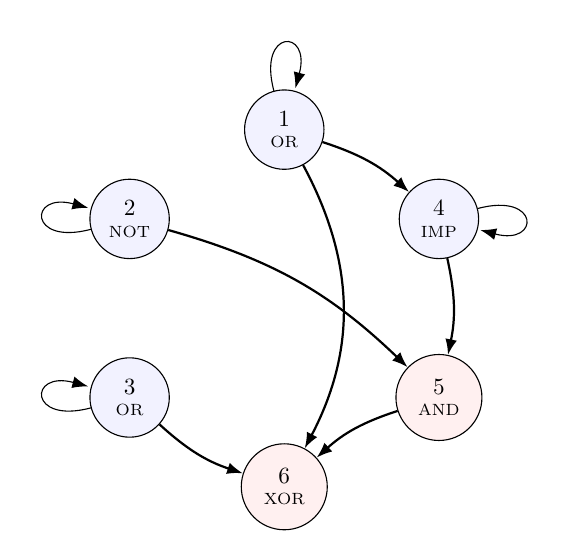
\begin{tikzpicture}[
  scale=0.84,
  transform shape,
  gate/.style={circle, draw, minimum size=12mm, align=center, inner sep=1pt, fill=blue!5},
  target/.style={circle, draw, minimum size=13mm, align=center, inner sep=1pt, fill=red!6},
  >={Latex[length=2mm]}
]
\node[gate] (n1) at (90:2.7) {1\\[-1mm]\scriptsize OR};
\node[gate] (n2) at (150:2.7) {2\\[-1mm]\scriptsize NOT};
\node[gate] (n3) at (210:2.7) {3\\[-1mm]\scriptsize OR};
\node[gate] (n4) at (30:2.7) {4\\[-1mm]\scriptsize IMP};
\node[target] (n5) at (-30:2.7) {5\\[-1mm]\scriptsize AND};
\node[target] (n6) at (-90:2.7) {6\\[-1mm]\scriptsize XOR};
\draw[->] (n1) edge[loop above] ();
\draw[->] (n2) edge[loop left] ();
\draw[->] (n3) edge[loop left] ();
\draw[->] (n4) edge[loop right] ();
\draw[->, thick] (n1) to[bend left=12] (n4);
\draw[->, thick] (n2) to[bend left=14] (n5);
\draw[->, thick] (n4) to[bend left=12] (n5);
\draw[->, thick] (n1) to[bend left=28] (n6);
\draw[->, thick] (n3) to[bend right=12] (n6);
\draw[->, thick] (n5) to[bend right=12] (n6);
\end{tikzpicture}
\end{adjustbox}
\caption{Six-node corroboration network. Nodes~1--4 (blue) provide inputs; nodes~5 and~6 (red) are the targets of the AND and XOR corroboration, respectively. Edge directions follow the connectivity matrix \(cm^{(\mathrm{corr})}\) in Figure~\ref{fig:corroboration-matrices}.}
\label{fig:corroboration-network}
\end{figure}

\small
\textbf{Corroboration pipeline.}
\[
\begin{aligned}
\{11\},\ \Omega(I_{nc})
&=\{0,1,4,5,16,17,20,21,32,33,36,37,48,49,52,53\},\\
\operatorname{Dec}\bigl(\{11\},\Omega(I_{nc})\bigr)
&=\J_5^{\mathrm{AND}},\\
\J_5^{\mathrm{AND}}
&=\{11,12,15,16,27,28,31,32,43,44,47,48,59,60,63,64\},\\
\{2,4,5,7,10,11,13,16\},\ \{0,16,32,48\}
&\leadsto \J_6^{\mathrm{XOR}},\\
\operatorname{Dec}\bigl(\{2,4,5,7,10,11,13,16\},\{0,16,32,48\}\bigr)
&=\J_6^{\mathrm{XOR}},\\
\J_6^{\mathrm{XOR}}
&=\{j\in\U : y_6(j)=1\}.
\end{aligned}
\]

\normalsize

The shared exhaustive table~\ref{tab:corroboration-exhaustive} and Algorithm~\ref{alg:deconvolution} confirm exactly these analytically predicted indices.

\begin{table}[p]
\centering
\setlength{\tabcolsep}{2pt}
\renewcommand{\arraystretch}{0.83}
\tiny
\begin{adjustbox}{max totalsize={\textwidth}{0.84\textheight},center}
\begin{tabular}{@{}rcccc@{}}
\toprule
\(j\) & Input Vector \(x\) & Output Vector \(F(x)\) & \(y_5\) & \(y_6\)\\
\midrule
1 & \texttt{000000} & \texttt{010100} & 0 & 0 \\
2 & \texttt{100000} & \texttt{110001} & 0 & \textbf{\textcolor{blue}{1}} \\
3 & \texttt{010000} & \texttt{000100} & 0 & 0 \\
4 & \texttt{110000} & \texttt{100001} & 0 & \textbf{\textcolor{blue}{1}} \\
5 & \texttt{001000} & \texttt{011101} & 0 & \textbf{\textcolor{blue}{1}} \\
6 & \texttt{101000} & \texttt{111000} & 0 & 0 \\
7 & \texttt{011000} & \texttt{001101} & 0 & \textbf{\textcolor{blue}{1}} \\
8 & \texttt{111000} & \texttt{101000} & 0 & 0 \\
9 & \texttt{000100} & \texttt{010100} & 0 & 0 \\
10 & \texttt{100100} & \texttt{110101} & 0 & \textbf{\textcolor{blue}{1}} \\
11 & \texttt{010100} & \texttt{000111} & \textbf{\textcolor{red}{1}} & \textbf{\textcolor{blue}{1}} \\
12 & \texttt{110100} & \texttt{100110} & \textbf{\textcolor{red}{1}} & 0 \\
13 & \texttt{001100} & \texttt{011101} & 0 & \textbf{\textcolor{blue}{1}} \\
14 & \texttt{101100} & \texttt{111100} & 0 & 0 \\
15 & \texttt{011100} & \texttt{001110} & \textbf{\textcolor{red}{1}} & 0 \\
16 & \texttt{111100} & \texttt{101111} & \textbf{\textcolor{red}{1}} & \textbf{\textcolor{blue}{1}} \\
17 & \texttt{000010} & \texttt{010100} & 0 & 0 \\
18 & \texttt{100010} & \texttt{110001} & 0 & \textbf{\textcolor{blue}{1}} \\
19 & \texttt{010010} & \texttt{000100} & 0 & 0 \\
20 & \texttt{110010} & \texttt{100001} & 0 & \textbf{\textcolor{blue}{1}} \\
21 & \texttt{001010} & \texttt{011101} & 0 & \textbf{\textcolor{blue}{1}} \\
22 & \texttt{101010} & \texttt{111000} & 0 & 0 \\
23 & \texttt{011010} & \texttt{001101} & 0 & \textbf{\textcolor{blue}{1}} \\
24 & \texttt{111010} & \texttt{101000} & 0 & 0 \\
25 & \texttt{000110} & \texttt{010100} & 0 & 0 \\
26 & \texttt{100110} & \texttt{110101} & 0 & \textbf{\textcolor{blue}{1}} \\
27 & \texttt{010110} & \texttt{000111} & \textbf{\textcolor{red}{1}} & \textbf{\textcolor{blue}{1}} \\
28 & \texttt{110110} & \texttt{100110} & \textbf{\textcolor{red}{1}} & 0 \\
29 & \texttt{001110} & \texttt{011101} & 0 & \textbf{\textcolor{blue}{1}} \\
30 & \texttt{101110} & \texttt{111100} & 0 & 0 \\
31 & \texttt{011110} & \texttt{001110} & \textbf{\textcolor{red}{1}} & 0 \\
32 & \texttt{111110} & \texttt{101111} & \textbf{\textcolor{red}{1}} & \textbf{\textcolor{blue}{1}} \\
33 & \texttt{000001} & \texttt{010100} & 0 & 0 \\
34 & \texttt{100001} & \texttt{110001} & 0 & \textbf{\textcolor{blue}{1}} \\
35 & \texttt{010001} & \texttt{000100} & 0 & 0 \\
36 & \texttt{110001} & \texttt{100001} & 0 & \textbf{\textcolor{blue}{1}} \\
37 & \texttt{001001} & \texttt{011101} & 0 & \textbf{\textcolor{blue}{1}} \\
38 & \texttt{101001} & \texttt{111000} & 0 & 0 \\
39 & \texttt{011001} & \texttt{001101} & 0 & \textbf{\textcolor{blue}{1}} \\
40 & \texttt{111001} & \texttt{101000} & 0 & 0 \\
41 & \texttt{000101} & \texttt{010100} & 0 & 0 \\
42 & \texttt{100101} & \texttt{110101} & 0 & \textbf{\textcolor{blue}{1}} \\
43 & \texttt{010101} & \texttt{000111} & \textbf{\textcolor{red}{1}} & \textbf{\textcolor{blue}{1}} \\
44 & \texttt{110101} & \texttt{100110} & \textbf{\textcolor{red}{1}} & 0 \\
45 & \texttt{001101} & \texttt{011101} & 0 & \textbf{\textcolor{blue}{1}} \\
46 & \texttt{101101} & \texttt{111100} & 0 & 0 \\
47 & \texttt{011101} & \texttt{001110} & \textbf{\textcolor{red}{1}} & 0 \\
48 & \texttt{111101} & \texttt{101111} & \textbf{\textcolor{red}{1}} & \textbf{\textcolor{blue}{1}} \\
49 & \texttt{000011} & \texttt{010100} & 0 & 0 \\
50 & \texttt{100011} & \texttt{110001} & 0 & \textbf{\textcolor{blue}{1}} \\
51 & \texttt{010011} & \texttt{000100} & 0 & 0 \\
52 & \texttt{110011} & \texttt{100001} & 0 & \textbf{\textcolor{blue}{1}} \\
53 & \texttt{001011} & \texttt{011101} & 0 & \textbf{\textcolor{blue}{1}} \\
54 & \texttt{101011} & \texttt{111000} & 0 & 0 \\
55 & \texttt{011011} & \texttt{001101} & 0 & \textbf{\textcolor{blue}{1}} \\
56 & \texttt{111011} & \texttt{101000} & 0 & 0 \\
57 & \texttt{000111} & \texttt{010100} & 0 & 0 \\
58 & \texttt{100111} & \texttt{110101} & 0 & \textbf{\textcolor{blue}{1}} \\
59 & \texttt{010111} & \texttt{000111} & \textbf{\textcolor{red}{1}} & \textbf{\textcolor{blue}{1}} \\
60 & \texttt{110111} & \texttt{100110} & \textbf{\textcolor{red}{1}} & 0 \\
61 & \texttt{001111} & \texttt{011101} & 0 & \textbf{\textcolor{blue}{1}} \\
62 & \texttt{101111} & \texttt{111100} & 0 & 0 \\
63 & \texttt{011111} & \texttt{001110} & \textbf{\textcolor{red}{1}} & 0 \\
64 & \texttt{111111} & \texttt{101111} & \textbf{\textcolor{red}{1}} & \textbf{\textcolor{blue}{1}} \\
\bottomrule
\end{tabular}
\end{adjustbox}
\caption{Exhaustive corroboration table for the six-node network under LSB-first ordering. Bold red entries in the \(y_5\) column mark the analytically predicted indices in \(\J_5^{\mathrm{AND}}\); bold blue entries in the \(y_6\) column mark the analytically predicted indices in \(\J_6^{\mathrm{XOR}}\). Rows containing both highlights are exactly the repertoire positions at which the composed XOR node is active while the intermediate AND node is also active.}
\label{tab:corroboration-exhaustive}
\end{table}



\begin{algorithm}[H]
\caption{Exact one-set deconvolution}\label{alg:deconvolution}
\KwIn{Connected-input set $\Ic$, network size $n$, ordering policy}
\KwOut{Exact one-set $\J$}
Compute decimal anchor $P(\Ic) = \sum_{i \in \Ic} w(i)$\;
Compute free set $I_{nc} = \{1,\dots,n\} \setminus \Ic$\;
Enumerate offset family $\Omega(I_{nc}) = \{\Delta_{nc}(\eta) : \eta \in \{0,1\}^{|I_{nc}|}\}$\;
Compute base set $L = \{1 + P(\Ic)\}$\;
\Return{$\J = \operatorname{Dec}(L, \Omega(I_{nc}))$}
\end{algorithm}


The analytic formula and the exhaustive table are two encodings of the same one-set. The formula
\[
\J_5^{\mathrm{AND}}=\operatorname{Dec}\bigl(\{11\},\Omega(I_{nc})\bigr),
\qquad
\Omega(I_{nc})=\{0,1,4,5,16,17,20,21,32,33,36,37,48,49,52,53\},
\]
gives the causal law in closed form. Deconvolution unfolds it to the explicit index list
\[
\{11,12,15,16,27,28,31,32,43,44,47,48,59,60,63,64\},
\]
which are precisely the rows of Table~\ref{tab:corroboration-exhaustive} where the fifth output column equals~\(1\).


\subsubsection{XOR case}
The XOR case uses the same six-node network shown in Figure~\ref{fig:corroboration-network}.
\[
y_6=x_1\oplus x_3\oplus (x_2\land x_4).
\]
Holding \(x_5\) and \(x_6\) free leaves the four-bit base repertoire
\[
L_{\mathrm{XOR}}=\{2,4,5,7,10,11,13,16\},
\qquad
\Omega(\{5,6\})=\{0,16,32,48\},
\]
so that
\[
\J_6^{\mathrm{XOR}}
=
\operatorname{Dec}\bigl(L_{\mathrm{XOR}},\Omega(\{5,6\})\bigr).
\]
After deconvolution, this gives
\[
\begin{aligned}
\J_6^{\mathrm{XOR}}=
\{&2,4,5,7,10,11,13,16,18,20,21,23,26,27,29,32,\\
&34,36,37,39,42,43,45,48,50,52,53,55,58,59,61,64\}.
\end{aligned}
\]
This confirms that the formalism does not depend on monotonicity.
In Table~\ref{tab:corroboration-exhaustive},
the blue entries coincide exactly with this one-set, showing that the
same calculus recovers parity-based behaviour as well.

\subsubsection{Multiple Gates Interaction and Exact Reconstruction}
We now consider the case of multiple interacting nodes of distinct families,
resulting in simultaneous satisfaction of several heterogeneous constraints.

For this example, consider the 10-node case described in fig~\ref{fig:mixed10-ring}. 
Its local input sets and exact one-set formulas are shown in table~\ref{tab:mixed10-node-formulas}.

\begin{table}[H]
\centering
\small
\begin{tabular}{@{}ccp{0.55\linewidth}@{}}
\toprule
\textbf{Node \(i\)} & \textbf{Input set \(N_i\)} & \textbf{One-set formula \(\J_i\)} \\
\midrule
1 & \(\{2,3\}\) & \(\Band{2}{1}\cap\Band{3}{1}\) \\
2 & \(\{1,3\}\) & \(\Band{1}{1}\cup\Band{3}{1}\) \\
3 & \(\{4,5\}\) & \(\Parity{\{4,5\}}{1}\) \\
4 & \(\{2,3,5\}\) & \(\Weight{\{2,3,5\}}{2}\cup\Weight{\{2,3,5\}}{3}\) \\
5 & \(\{6\}\) & \(\Band{6}{0}\) \\
6 & \(\{5,7\}\) & \(\Parity{\{5,7\}}{0}\) \\
7 & \(\{6\}\) & \(\Band{6}{0}\) \\
8 & \(\{1,9\}\) & \(\U\setminus\bigl(\Band{1}{1}\cap\Band{9}{0}\bigr)\) \\
9 & \(\{2,10\}\) & \(\Band{2}{1}\cap\Band{10}{0}\) \\
10 & \(\{3,4,7,8\}\) & \(\Weight{\{3,4,7,8\}}{3}\cup\Weight{\{3,4,7,8\}}{4}\) \\
\bottomrule
\end{tabular}
\caption{Local input sets and analytic one-set formulas for all 10 nodes 
in the mixed benchmark network.}
\label{tab:mixed10-node-formulas}
\end{table}


Here node \(4\) is a \(2\)-of-\(3\) threshold gate and node \(10\) is a strict majority gate on four inputs. 
Notice that the network is not homogeneous: monotone, parity, negation, implication, 
and threshold mechanisms coexist in the same causal object.



\begin{figure}[t]
\centering
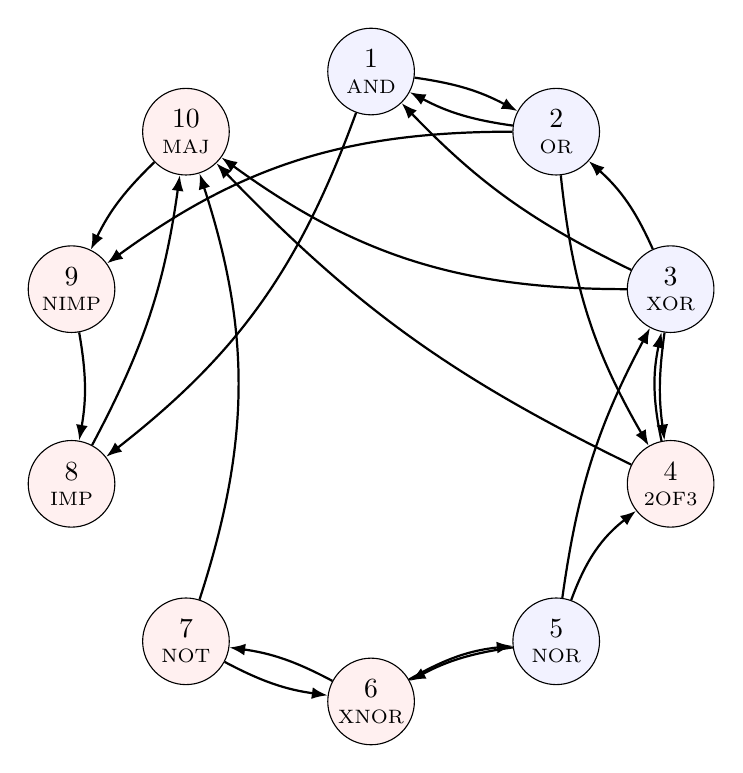
\begin{tikzpicture}[
  gate/.style={circle, draw, minimum size=11mm, align=center, inner sep=1pt, fill=blue!5},
  focus/.style={circle, draw, minimum size=11mm, align=center, inner sep=1pt, fill=red!6},
  >={Latex[length=2mm]}
]
\node[gate]  (n1)  at (90:4.0)   {1\\[-1mm]\scriptsize AND};
\node[gate]  (n2)  at (54:4.0)   {2\\[-1mm]\scriptsize OR};
\node[gate]  (n3)  at (18:4.0)   {3\\[-1mm]\scriptsize XOR};
\node[focus] (n4)  at (-18:4.0)  {4\\[-1mm]\scriptsize 2OF3};
\node[gate]  (n5)  at (-54:4.0)  {5\\[-1mm]\scriptsize NOR};
\node[focus] (n6)  at (-90:4.0)  {6\\[-1mm]\scriptsize XNOR};
\node[focus] (n7)  at (-126:4.0) {7\\[-1mm]\scriptsize NOT};
\node[focus] (n8)  at (-162:4.0) {8\\[-1mm]\scriptsize IMP};
\node[focus] (n9)  at (162:4.0)  {9\\[-1mm]\scriptsize NIMP};
\node[focus] (n10) at (126:4.0)  {10\\[-1mm]\scriptsize MAJ};

\draw[->, thick] (n2) to[bend left=10] (n1);
\draw[->, thick] (n3) to[bend left=10] (n1);
\draw[->, thick] (n1) to[bend left=10] (n2);
\draw[->, thick] (n3) to[bend right=12] (n2);
\draw[->, thick] (n4) to[bend left=12] (n3);
\draw[->, thick] (n5) to[bend left=10] (n3);
\draw[->, thick] (n2) to[bend right=12] (n4);
\draw[->, thick] (n3) to[bend right=8] (n4);
\draw[->, thick] (n5) to[bend left=16] (n4);
\draw[->, thick] (n6) to[bend left=12] (n5);
\draw[->, thick] (n5) to[bend right=10] (n6);
\draw[->, thick] (n7) to[bend right=10] (n6);
\draw[->, thick] (n6) to[bend right=10] (n7);
\draw[->, thick] (n1) to[bend left=16] (n8);
\draw[->, thick] (n9) to[bend left=10] (n8);
\draw[->, thick] (n2) to[bend right=18] (n9);
\draw[->, thick] (n10) to[bend right=10] (n9);
\draw[->, thick] (n3) to[bend left=18] (n10);
\draw[->, thick] (n4) to[bend left=10] (n10);
\draw[->, thick] (n7) to[bend right=18] (n10);
\draw[->, thick] (n8) to[bend right=10] (n10);
\end{tikzpicture}
\caption{Ten-node mixed-gate benchmark network. Blue nodes use monotone or parity gates; red nodes use threshold, negation, implication, or majority gates. The heterogeneous gate mixture is the basis for the overlap and dynamical analyses that follow.}
\label{fig:mixed10-ring}
\end{figure}

\begin{definition}[Analytic Predictor]
For each node \(i\), let \(\J_i\subseteq\U\) denote the one-set determined by its gate family, parameters, connected-input set \(N_i\), and the declared ordering policy. The analytic predictor reconstructs the network output matrix \(Y\in\bits^{2^n\times n}\) by declaring
\[
Y_{j,i}=1 \iff j\in \J_i.
\]
\end{definition}

\begin{theorem}[Canonical Exact Reconstruction]\label{thm:canonical-reconstruction}
Fix a network \((cm,dynamic)\), its gate parameters, and an ordering policy. Then the analytic predictor coincides exactly with the exhaustive one-step synchronous baseline:
\[
Y^{\mathrm{analytic}}=Y^{\mathrm{baseline}}.
\]
\end{theorem}

\begin{proof}
Fix a repertoire index \(j\in\U\) and a node \(i\in\{1,\ldots,n\}\). The baseline entry is \(Y^{\mathrm{baseline}}_{j,i}=g_i(x_{N_i}(j))\), where \(x_{N_i}(j)\) denotes the restriction of the \(j\)-th input vector to the connected-input set \(N_i\). By Proposition~\ref{prop:gate-family-one-sets}, the gate predicate \(g_i\) evaluates to one on input \(x_{N_i}(j)\) if and only if \(j\in\J_i\), where \(\J_i\) is the one-set corresponding to the gate family of node \(i\). The analytic entry is \(Y^{\mathrm{analytic}}_{j,i}=\mathbf{1}[j\in\J_i]\) by definition. Therefore \(Y^{\mathrm{analytic}}_{j,i}=Y^{\mathrm{baseline}}_{j,i}\) for every \(j\) and every \(i\), and equality of all entries implies \(Y^{\mathrm{analytic}}=Y^{\mathrm{baseline}}\).
\end{proof}

The theorem is best read operationally. It does not claim that the \(2^n\) states disappear. It claims that the full behaviour of a heterogeneous network can be reconstructed from short local causal formulas without recomputing every row gate by gate.

The central point for mixed queries is that overlap is not a nuisance but a source of analytic compression. 
If several queried gates reuse some of the same input coordinates, then the final query does not depend 
on the sum of their local arities as if those gates were independent objects. It depends only on the 
union of the coordinates that actually appear across the queried mechanisms due to overlap, 
the distribution-of-information becomes mathematically precise: repeated 
coordinates are not recomputed as new information; they are shared constraints propagated 
through several local laws.

To show the propagation of overlap constraints, in the following sections are analyzed six 
cases based in the network described in
 Figure~\ref{fig:mixed10-ring}.
Four of them are 
full-output queries on all ten nodes. Two are subsystem queries on selected nodes only. 

The four full-output cases called as \(\J_{\mathrm{F1,F2,F3,F4}}\) are:
\[
\begin{aligned}
\J_{\mathrm{F1}}&=\bigcap_{i=1}^{10}\J_i,\\
\J_{\mathrm{F2}}&=\Bigl(\bigcap_{i=1}^{9}\J_i\Bigr)\cap(\U\setminus\J_{10}),\\
\J_{\mathrm{F3}}&=\Bigl(\bigcap_{i\in\{1,\dots,8,10\}}\J_i\Bigr)\cap(\U\setminus\J_{9}),\\
\J_{\mathrm{F4}}&=\Bigl(\bigcap_{i\in\{1,2,3,4,5,7,8,9,10\}}\J_i\Bigr)\cap(\U\setminus\J_{6}).
\end{aligned}
\]
The two subsystem queries called as \(\J_{\mathrm{S1,S2}}\) are:
\[
\begin{aligned}
\J_{\mathrm{S1}}
&=(\U\setminus\J_4)\cap \J_6\cap \J_7\cap \J_{10},\\
\J_{\mathrm{S2}}
&=(\U\setminus\J_4)\cap \J_6\cap \J_7\cap \J_8\cap (\U\setminus\J_9)\cap \J_{10}.
\end{aligned}
\]
Case \(\J_{\mathrm{S1}}\) mixes threshold, parity, negation, and majority constraints. 
Case \(\J_{\mathrm{S2}}\) goes further by adding implication and the complement of a 
non-implication condition. In both cases the queried event is an exact intersection 
of heterogeneous causal laws over overlapping coordinates.

\begin{definition}[Query Support Union]
For a query \(q=(Q,\sigma)\), where \(Q\subseteq [n]\) is the set of queried nodes and \(\sigma\in\bits^{|Q|}\) is the target output pattern, define
\[
C_q=\bigcup_{i\in Q}N_i,
\qquad
F_q=[n]\setminus C_q.
\]
The set \(C_q\) is the \emph{query support union}: the coordinates whose values can affect the truth of the query. The complementary set \(F_q\) contains coordinates that are free for that query.
\end{definition}

\begin{proposition}[Overlap-Supported Query Factorisation]\label{prop:overlap-factorisation}
Let
\[
\J_q=\bigcap_{i\in Q^+}\J_i \cap \bigcap_{i\in Q^-}(\U\setminus\J_i)
\]
be any exact mixed query, where \(Q^+\) and \(Q^-\) are the queried nodes constrained to output \(1\) and \(0\), respectively. Then:
\[
x|_{C_q}=x'|_{C_q}\quad \Longrightarrow \quad \bigl(x\in \J_q \iff x'\in \J_q\bigr).
\]
Equivalently, if
\[
L_q^{(0)}=\{j\in \J_q : x_k(j)=0 \text{ for every } k\in F_q\},
\]
then
\[
\J_q=\operatorname{Dec}\bigl(L_q^{(0)},\Omega(F_q)\bigr).
\]
\end{proposition}

\begin{proof}
Each local condition \(\J_i\) or \(\U\setminus\J_i\) depends only on the coordinates in \(N_i\). 
Therefore the full query \(\J_q\), being an intersection of such conditions, depends 
only on the coordinates in the union \(C_q=\bigcup_{i\in Q}N_i\). 
Changing any coordinate in \(F_q\) leaves the truth of all local conditions unchanged. 
Hence every satisfying assignment on \(C_q\) lifts uniformly across all offsets 
generated by the free coordinates \(F_q\), which is exactly the 
deconvolution \(\operatorname{Dec}(L_q^{(0)},\Omega(F_q))\).
\end{proof}

\begin{corollary}[Exact Reduction From Shared Inputs]\label{cor:shared-input-reduction}
Let
\[
d_q=\sum_{i\in Q}|N_i|,
\qquad
c_q=|C_q|,
\qquad
\mu_q=d_q-c_q.
\]
If the queried local conditions were enumerated independently, the raw 
local-assignment space would 
have size \(2^{d_q}\). After overlap consolidation, 
only \(2^{c_q}\) compatible assignments on \(C_q\) remain. 
Hence the exact reduction factor is
\[
R_q=2^{\mu_q}=2^{d_q-c_q}.
\]
Equality \(\mu_q=0\) occurs only when the queried input sets are pairwise disjoint. Every shared coordinate increases \(\mu_q\) through inclusion-exclusion and therefore enlarges the reduction factor.
\end{corollary}

This shows that overlap has an exact combinatorial value. The query does not pay once
 per gate for a shared coordinate; it pays once for the coordinate itself. In
 that sense the queried information is distributed hierarchically across the network: 
 one coordinate can constrain several local mechanisms simultaneously. 
 
% They do not yet justify a 
% stronger claim of full mathematical fractality, so witse restricted to the exact
% overlap statement proved above.

\begin{figure}[H]
\centering
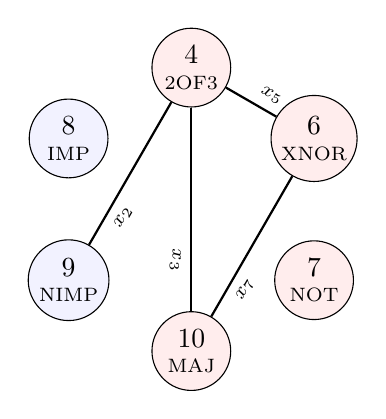
\begin{tikzpicture}[
  qnode/.style={circle, draw, minimum size=10mm, align=center, inner sep=1pt, fill=blue!5},
  core/.style={circle, draw, minimum size=10mm, align=center, inner sep=1pt, fill=red!7},
  >={Latex[length=2mm]}
]
% Nodes arranged in a symmetric ring with radius 1.8cm
\node[core]  (q4)  at (90:1.8)  {4\\[-1mm]\scriptsize 2OF3};    % Top (core/S1 node)
\node[qnode] (q8)  at (150:1.8) {8\\[-1mm]\scriptsize IMP};   % Upper left (S2-only node)
\node[qnode] (q9)  at (210:1.8) {9\\[-1mm]\scriptsize NIMP};  % Lower left (S2-only node)
\node[core]  (q10) at (270:1.8) {10\\[-1mm]\scriptsize MAJ};  % Bottom (core/S1 node)
\node[core]  (q7)  at (330:1.8) {7\\[-1mm]\scriptsize NOT};   % Lower right (core/S1 node)
\node[core]  (q6)  at (30:1.8)  {6\\[-1mm]\scriptsize XNOR};  % Upper right (core/S1 node)

% Draw edges with shared input coordinate labels
\draw[-, thick] (q4) -- node[sloped, above, near end] {\scriptsize \(x_5\)} (q6);
\draw[-, thick] (q4) -- node[sloped, below, near end] {\scriptsize \(x_2\)} (q9);
\draw[-, thick] (q6) -- node[sloped, below, near end] {\scriptsize \(x_7\)} (q10);
\draw[-, thick] (q4) -- node[sloped, below, near end] {\scriptsize \(x_3\)} (q10);
\end{tikzpicture}
\caption{Overlap graph for the mixed queries. Red nodes form the four-gate subsystem query \(S1\); adding nodes \(8\) and \(9\) gives \(S2\). Edge labels indicate the exact shared input coordinates. The graph makes the combinatorial source of the reduction factor explicit: coordinates \(x_2,x_3,x_5,x_7\) are reused across several queried mechanisms rather than treated independently.}
\label{fig:mixed10-overlap}
\end{figure}

\begin{table}[H]
\centering
\setlength{\tabcolsep}{4pt}
\scriptsize
\begin{adjustbox}{max width=\textwidth,center}
\begin{tabular}{@{}lccccccl@{}}
\toprule
Case & Queried Nodes & \(d_q\) & \(c_q\) & \(\mu_q\) & \(R_q\) & \(F_q\) & \(C_q\)\\
\midrule
F1--F4 & \(\{1,\dots,10\}\) & 21 & 10 & 11 & \(2^{11}=2048\) & \(\varnothing\) & \(\{1,\dots,10\}\) \\
S1 & \(\{4,6,7,10\}\) & 10 & 7 & 3 & \(2^3=8\) & \(\{1,9,10\}\) & \(\{2,3,4,5,6,7,8\}\) \\
S2 & \(\{4,6,7,8,9,10\}\) & 14 & 10 & 4 & \(2^4=16\) & \(\varnothing\) & \(\{1,\dots,10\}\) \\
\bottomrule
\end{tabular}
\end{adjustbox}
\caption{Exact overlap statistics for the mixed queries. The quantity \(d_q\) is the sum of queried gate arities, \(c_q\) is the size of the union of their input coordinates, \(\mu_q=d_q-c_q\) measures repeated coordinate use, and \(R_q=2^{\mu_q}\) is the exact reduction factor in the raw local-assignment space.}
\label{tab:mixed10-overlap-stats}
\end{table}

The most transparent case is \(S1\). As is shown in second row of Table~\ref{tab:mixed10-overlap-stats},
\[
C_{\mathrm{S1}}=\{2,3,4,5,6,7,8\},
\qquad
F_{\mathrm{S1}}=\{1,9,10\},
\]
so the query depends on only seven determining coordinates even though the four queried gates contribute \(3+2+1+4=10\) local inputs in total. The free coordinates produce the exact offset family
\[
\Omega(F_{\mathrm{S1}})=\{0,1,256,257,512,513,768,769\},
\]
and the zero-free base set is
\[
L_{\mathrm{S1}}^{(0)}=\{141,217\}.
\]
Therefore
\[
\J_{\mathrm{S1}}=
\operatorname{Dec}\bigl(\{141,217\},\Omega(\{1,9,10\})\bigr),
\]
which unfolds to the 16 corroborated rows listed later in Table~\ref{tab:mixed10-subsystem-rows}. 
This is the exact mixed-gate analogue of the detailed AND deconvolution: 
overlap first shrinks the determining coordinate set, and only then do 
the remaining free coordinates generate the full family of offsets.

\begin{table}[H]
\centering
\setlength{\tabcolsep}{3pt}
\scriptsize
\begin{adjustbox}{max width=\textwidth,center}
\begin{tabular}{@{}lccccc@{}}
\toprule
Case & Output Pattern & Anchor \(j_0\) & Offsets \(\Omega_q\) & Unfolded Indices \(\J_q\) & Rows\\
\midrule
F1 & \texttt{1111111111} & 143 & \(\{0,72,256,257,328,329\}\) & \(\{143,215,399,400,471,472\}\) & 6 \\
F2 & \texttt{1111111110} & 15 & \(\{0,72,256,257,328,329\}\) & \(\{15,87,271,272,343,344\}\) & 6 \\
F3 & \texttt{1111111101} & 655 & \(\{0,72,256,257,328,329\}\) & \(\{655,727,911,912,983,984\}\) & 6 \\
F4 & \texttt{1111101111} & 79 & \(\{0,128,256,257,384,385\}\) & \(\{79,207,335,336,463,464\}\) & 6 \\
\bottomrule
\end{tabular}
\end{adjustbox}
\caption{Analytic unfolding summary for the four full-output queries on the 10-node benchmark. Each case is defined by an exact global output pattern, an anchor index, and the offset family that unfolds to the full set of satisfying repertoire positions.}
\label{tab:mixed10-full-summary}
\end{table}

\begin{table}[H]
\centering
\setlength{\tabcolsep}{3pt}
\scriptsize
\begin{adjustbox}{max width=\textwidth,center}
\begin{tabular}{@{}lcccccc@{}}
\toprule
Case & Queried Nodes & Projection & Anchor \(j_0\) & Offsets \(\Omega_q\) & Unfolded Indices \(\J_q\) & Rows\\
\midrule
S1 & \(\{4,6,7,10\}\) & \texttt{0111} & 141 & \(\{0,1,76,77,256,257,332,333,512,513,588,589,768,769,844,845\}\) & \(\{141,142,217,218,397,398,473,474,653,654,729,730,909,910,985,986\}\) & 16 \\
S2 & \(\{4,6,7,8,9,10\}\) & \texttt{011101} & 141 & \(\{0,76,256,257,332,333,512,588,768,769,844,845\}\) & \(\{141,217,397,398,473,474,653,729,909,910,985,986\}\) & 12 \\
\bottomrule
\end{tabular}
\end{adjustbox}
\caption{Analytic unfolding summary for the subsystem queries. The first case keeps four heterogeneous constraints, while the second keeps six. Relaxing the query from the full 10-bit output to a subsystem increases support, but the resulting indices are still obtained analytically rather than by exhaustive scanning.}
\label{tab:mixed10-subsystem-summary}
\end{table}


\begin{table}[H]
\centering
\setlength{\tabcolsep}{4pt}
\footnotesize
\begin{adjustbox}{max width=\textwidth,center}
\begin{tabular}{@{}lrcc@{}}
\toprule
Case & \(j\) & Input Vector \(x\) & Output Vector \(F(x)\)\\
\midrule
F1 & 143 & \texttt{0111000100} & \texttt{1111111111} \\
F1 & 215 & \texttt{0110101100} & \texttt{1111111111} \\
F1 & 399 & \texttt{0111000110} & \texttt{1111111111} \\
F1 & 400 & \texttt{1111000110} & \texttt{1111111111} \\
F1 & 471 & \texttt{0110101110} & \texttt{1111111111} \\
F1 & 472 & \texttt{1110101110} & \texttt{1111111111} \\
F2 & 15 & \texttt{0111000000} & \texttt{1111111110} \\
F2 & 87 & \texttt{0110101000} & \texttt{1111111110} \\
F2 & 271 & \texttt{0111000010} & \texttt{1111111110} \\
F2 & 272 & \texttt{1111000010} & \texttt{1111111110} \\
F2 & 343 & \texttt{0110101010} & \texttt{1111111110} \\
F2 & 344 & \texttt{1110101010} & \texttt{1111111110} \\
F3 & 655 & \texttt{0111000101} & \texttt{1111111101} \\
F3 & 727 & \texttt{0110101101} & \texttt{1111111101} \\
F3 & 911 & \texttt{0111000111} & \texttt{1111111101} \\
F3 & 912 & \texttt{1111000111} & \texttt{1111111101} \\
F3 & 983 & \texttt{0110101111} & \texttt{1111111101} \\
F3 & 984 & \texttt{1110101111} & \texttt{1111111101} \\
F4 & 79 & \texttt{0111001000} & \texttt{1111101111} \\
F4 & 207 & \texttt{0111001100} & \texttt{1111101111} \\
F4 & 335 & \texttt{0111001010} & \texttt{1111101111} \\
F4 & 336 & \texttt{1111001010} & \texttt{1111101111} \\
F4 & 463 & \texttt{0111001110} & \texttt{1111101111} \\
F4 & 464 & \texttt{1111001110} & \texttt{1111101111} \\
\bottomrule
\end{tabular}
\end{adjustbox}
\caption{All satisfying rows for the four full-output cases. The table is not exhaustive over the full \(2^{10}=1024\) repertoire; it contains only the rows analytically predicted to satisfy each selected full pattern.}
\label{tab:mixed10-full-rows}
\end{table}

\begin{table}[H]
\centering
\setlength{\tabcolsep}{4pt}
\footnotesize
\begin{adjustbox}{max width=\textwidth,center}
\begin{tabular}{@{}lcrcc@{}}
\toprule
Case & Projection & \(j\) & Input Vector \(x\) & Output Vector \(F(x)\)\\
\midrule
S1 & \texttt{0111} & 141 & \texttt{0011000100} & \texttt{0110111101} \\
S1 & \texttt{0111} & 142 & \texttt{1011000100} & \texttt{0110111001} \\
S1 & \texttt{0111} & 217 & \texttt{0001101100} & \texttt{0000111101} \\
S1 & \texttt{0111} & 218 & \texttt{1001101100} & \texttt{0100111001} \\
S1 & \texttt{0111} & 397 & \texttt{0011000110} & \texttt{0110111101} \\
S1 & \texttt{0111} & 398 & \texttt{1011000110} & \texttt{0110111101} \\
S1 & \texttt{0111} & 473 & \texttt{0001101110} & \texttt{0000111101} \\
S1 & \texttt{0111} & 474 & \texttt{1001101110} & \texttt{0100111101} \\
S1 & \texttt{0111} & 653 & \texttt{0011000101} & \texttt{0110111101} \\
S1 & \texttt{0111} & 654 & \texttt{1011000101} & \texttt{0110111001} \\
S1 & \texttt{0111} & 729 & \texttt{0001101101} & \texttt{0000111101} \\
S1 & \texttt{0111} & 730 & \texttt{1001101101} & \texttt{0100111001} \\
S1 & \texttt{0111} & 909 & \texttt{0011000111} & \texttt{0110111101} \\
S1 & \texttt{0111} & 910 & \texttt{1011000111} & \texttt{0110111101} \\
S1 & \texttt{0111} & 985 & \texttt{0001101111} & \texttt{0000111101} \\
S1 & \texttt{0111} & 986 & \texttt{1001101111} & \texttt{0100111101} \\
S2 & \texttt{011101} & 141 & \texttt{0011000100} & \texttt{0110111101} \\
S2 & \texttt{011101} & 217 & \texttt{0001101100} & \texttt{0000111101} \\
S2 & \texttt{011101} & 397 & \texttt{0011000110} & \texttt{0110111101} \\
S2 & \texttt{011101} & 398 & \texttt{1011000110} & \texttt{0110111101} \\
S2 & \texttt{011101} & 473 & \texttt{0001101110} & \texttt{0000111101} \\
S2 & \texttt{011101} & 474 & \texttt{1001101110} & \texttt{0100111101} \\
S2 & \texttt{011101} & 653 & \texttt{0011000101} & \texttt{0110111101} \\
S2 & \texttt{011101} & 729 & \texttt{0001101101} & \texttt{0000111101} \\
S2 & \texttt{011101} & 909 & \texttt{0011000111} & \texttt{0110111101} \\
S2 & \texttt{011101} & 910 & \texttt{1011000111} & \texttt{0110111101} \\
S2 & \texttt{011101} & 985 & \texttt{0001101111} & \texttt{0000111101} \\
S2 & \texttt{011101} & 986 & \texttt{1001101111} & \texttt{0100111101} \\
\bottomrule
\end{tabular}
\end{adjustbox}
\caption{All satisfying rows for the subsystem queries. Here the projection column records the output pattern only on the selected nodes. The support enlarges from \(6\) to \(16\) or \(12\) rows because some global constraints are relaxed, but every row shown remains an exact analytic prediction corroborated against the exhaustive baseline.}
\label{tab:mixed10-subsystem-rows}
\end{table}

\paragraph{What changes when multiple gates are queried.}
In the single-gate AND example, the support has a simple rectangular structure: one decimal anchor plus an offset family induced by fully free coordinates. In the 10-node mixed queries, that geometry is constrained by overlap. Some cases, such as the full-output queries, have no free coordinates at all because \(C_q=[10]\), yet they still benefit strongly from overlap through Corollary~\ref{cor:shared-input-reduction}: the raw local-assignment space drops from \(2^{21}\) to \(2^{10}\), an exact reduction factor of \(2^{11}=2048\), before any row materialisation is considered. Others, such as \(S1\), benefit twice: first from overlap, which contracts the determining coordinates to seven; and then from deconvolution, which lifts the two base solutions across the three genuinely free coordinates. In the present benchmark, the four full-output queries all reduce to only six satisfying rows, and three of them share the same offset family
\[
\Omega_{\mathrm{full}}=\{0,72,256,257,328,329\},
\]
showing that different global output patterns can inherit the same combinatorial skeleton even when their terminal constraints differ. What appears in the full repertoire as dispersed behaviour is therefore explained analytically as overlap-aware reuse of shared coordinates and repeated offset blocks.


\begin{algorithm}[H]
\caption{Mixed-query evaluation}\label{alg:mixed-query}
\KwIn{Queried nodes $Q$, target pattern $\sigma$, connectivity $cm$, dynamics $dyn$}
\KwOut{Exact satisfying index set $\J_q$}
\For{each $i \in Q$}{Compute local one-set $\J_i$ via Proposition~\ref{prop:gate-family-one-sets}\;}
Compute support union $C_q = \bigcup_{i \in Q} N_i$\;
Compute free coordinates $F_q = [n] \setminus C_q$\;
Enumerate support-level assignments on $C_q$\;
Filter by intersection/complement conditions from $\sigma$\;
Compute base set $L_q^{(0)}$ from satisfying assignments with $F_q = \mathbf{0}$\;
Compute offset family $\Omega(F_q)$\;
\Return{$\J_q = \operatorname{Dec}(L_q^{(0)}, \Omega(F_q))$}
\end{algorithm}

These results are the counterpart of the analytic overlap treatment.
In the full-output queries, the offset family is \(\{0\}\) because
the support union fills all ten coordinates, leaving no free offsets
after intersection. In the \(S1\) query, by contrast, the
factorisation proved in Proposition~\ref{prop:overlap-factorisation} manifests directly:
the base set is \(\{141,217\}\), the free-coordinate offset family
is \(\{0,1,256,257,512,513,768,769\}\), and deconvolution
unfolds them to the 16 indices in \(\J_{\mathrm{S1}}\). In \(S2\), the
additional constraints saturate the coordinate union again, so the
offset family collapses to \(\{0\}\). In every case, exact equality
against the exhaustive dispatch baseline has been confirmed on all 1024
repertoire rows.


\subsubsection{Dynamical Landscape of the Same 10-Node Network}
The previous subsection answered an exact inverse question: which input rows produce the selected
mixed output events in Tables~\ref{tab:mixed10-full-summary} and~\ref{tab:mixed10-subsystem-summary}.
We now add the complementary forward-dynamical question on the same network:
which 10-bit patterns are themselves one-step realizable, and which belong to the recurrent
part of the state-transition graph?

Let \(F:\bits^{10}\to\bits^{10}\) be the synchronous update map induced by Figure~\ref{fig:mixed10-ring}.
Define the one-step image
\[
\Im(F)=F(\U),
\]
and let
\[
\operatorname{Attr}(F)=\{x\in\U:\exists p\ge 1 \text{ such that } F^p(x)=x\}
\]
be the recurrent set. Since \(\U\) is finite and \(F\) is deterministic, every state belongs to a unique
basin of attraction and eventually reaches a periodic orbit. This dynamical layer does not replace the
exact repertoire analysis above; rather, it situates those exact query outputs inside the broader
behavioural landscape generated by the same causal architecture.

Executed enumeration of all \(2^{10}=1024\) states gives
\[
|\Im(F)|=206,
\qquad
|\U\setminus\Im(F)|=818,
\qquad
\frac{|\Im(F)|}{|\U|}=\frac{206}{1024}\approx 0.201.
\]
Thus only about \(20.1\%\) of all 10-bit patterns are admissible as one-step outputs of the network.
This is a strong form of dynamical order: the local logical constraints described in
Table~\ref{tab:mixed10-node-formulas} and the overlap structure analysed in
Corollary~\ref{cor:shared-input-reduction} restrict the forward image to a small structured subset
of the full configuration space.

The recurrent dynamics collapse further. Table~\ref{tab:mixed10-attractor-summary} shows that the
entire functional graph has only four attractors: one fixed point, two 2-cycles, and one 6-cycle.
Their basin sizes sum to all 1024 states, and the three dominant basins
\[
488+320+204=1012
\]
already cover \(1012/1024\approx 98.8\%\) of the state space. The resulting picture is therefore not
one of undifferentiated combinatorial explosion, but of a highly constrained landscape in which many
exactly describable transient patterns feed a very small recurrent core.

\begin{figure}[t]
\centering
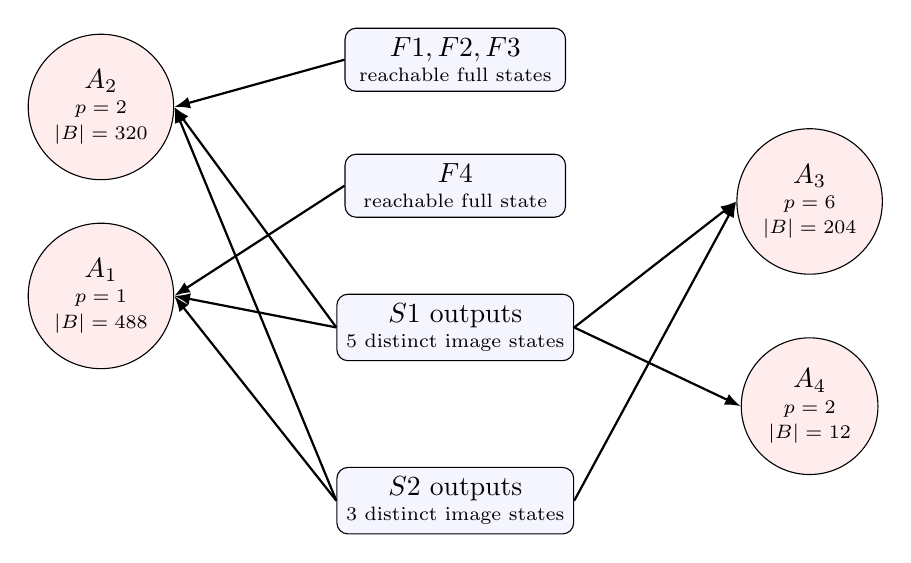
\begin{tikzpicture}[
  casebox/.style={draw, rounded corners, align=center, minimum width=28mm, minimum height=8mm, fill=blue!4},
  attractor/.style={draw, circle, align=center, minimum size=13mm, fill=red!7},
  >={Latex[length=2mm]}
]
% Left attractor column (first two attractors) - A2 moved down to increase separation from A1
\node[attractor] (a2) at (-4.5, 1.2) {\(A_2\)\\[-1mm]\scriptsize \(p=2\)\\[-1mm]\scriptsize \(|B|=320\)};
\node[attractor] (a1) at (-4.5, -1.2) {\(A_1\)\\[-1mm]\scriptsize \(p=1\)\\[-1mm]\scriptsize \(|B|=488\)};

% Middle case box column (all query cases) - adjusted to align with attractors
\node[casebox] (f123) at (0, 1.8) {\(F1,F2,F3\)\\[-1mm]\scriptsize reachable full states};
\node[casebox] (f4)   at (0, 0.2) {\(F4\)\\[-1mm]\scriptsize reachable full state};
\node[casebox] (s1)   at (0, -1.6) {\(S1\) outputs\\[-1mm]\scriptsize 5 distinct image states};
\node[casebox] (s2)   at (0, -3.8) {\(S2\) outputs\\[-1mm]\scriptsize 3 distinct image states};

% Right attractor column - A4 moved up to increase separation from A3
\node[attractor] (a3) at (4.5, -0.) {\(A_3\)\\[-1mm]\scriptsize \(p=6\)\\[-1mm]\scriptsize \(|B|=204\)};
\node[attractor] (a4) at (4.5, -2.6) {\(A_4\)\\[-1mm]\scriptsize \(p=2\)\\[-1mm]\scriptsize \(|B|=12\)};

% Draw arrows maintaining logical flow: left attractors <- case boxes -> right attractors
\draw[->, thick] (f123.west) -- (a2.east);
\draw[->, thick] (f4.west) -- (a1.east);
\draw[->, thick] (s1.west) -- (a1.east);
\draw[->, thick] (s1.west) -- (a2.east);
\draw[->, thick] (s1.east) -- (a3.west);
\draw[->, thick] (s1.east) -- (a4.west);
\draw[->, thick] (s2.west) -- (a1.east);
\draw[->, thick] (s2.west) -- (a2.east);
\draw[->, thick] (s2.east) -- (a3.west);
\end{tikzpicture}
\caption{Schematic condensation of the exact 10-node dynamical classification. The four full-output cases from Table~\ref{tab:mixed10-full-summary} and the subsystem outputs induced by Table~\ref{tab:mixed10-subsystem-summary} are all one-step reachable, but they distribute over only four eventual attractors. Adding the extra \(S2\) constraints removes the branch to \(A_4\), showing that stronger exact causal constraints reduce not only combinatorial freedom but also dynamical dispersion.}
\label{fig:mixed10-dynamical-schematic}
\end{figure}

\begin{table}[t]
\centering
\setlength{\tabcolsep}{5pt}
\scriptsize
\begin{adjustbox}{max width=\textwidth,center}
\begin{tabular}{@{}cccc@{}}
\toprule
Attractor & Period & Basin Size & Recurrent States \\
\midrule
\(A_1\) & 1 & 488 & \(\{0000010100\}\) \\
\(A_2\) & 2 & 320 & \(\{1101010110,0110010110\}\) \\
\(A_3\) & 6 & 204 & \(\{1111010101,1111010001,1111010000,1111010010,1111010110,1111010111\}\) \\
\(A_4\) & 2 & 12 & \(\{1111010100,1111010011\}\) \\
\bottomrule
\end{tabular}
\end{adjustbox}
\caption{Exact recurrent structure of the 10-node benchmark. Basin sizes were obtained by exhaustive functional-graph enumeration of the 1024 states.}
\label{tab:mixed10-attractor-summary}
\end{table}

\begin{table}[t]
\centering
\setlength{\tabcolsep}{4pt}
\scriptsize
\begin{adjustbox}{max width=\textwidth,center}
\begin{tabular}{@{}lccccccc@{}}
\toprule
Case & Type & Pattern & Status & Reachable & Recurrent & Eventual Attractor & Steps to Recurrence \\
\midrule
F1 & full & \texttt{1111111111} & state 1024 & yes & no & \(A_2\) & 3 \\
F2 & full & \texttt{1111111110} & state 512 & yes & no & \(A_2\) & 3 \\
F3 & full & \texttt{1111111101} & state 768 & yes & no & \(A_2\) & 3 \\
F4 & full & \texttt{1111101111} & state 992 & yes & no & \(A_1\) & 6 \\
S1 & subsystem & \texttt{0111} & 16 rows / 5 outputs & yes & no & \(\{A_1,A_2,A_3,A_4\}\) & --- \\
S2 & subsystem & \texttt{011101} & 12 rows / 3 outputs & yes & no & \(\{A_1,A_2,A_3\}\) & --- \\
\bottomrule
\end{tabular}
\end{adjustbox}
\caption{Dynamical status of the six analytically studied cases. Every selected pattern is one-step reachable, but none is itself recurrent. The full-output states collapse to one attractor class in three of the four cases, while the subsystem events span several basins because one local projection can still be compatible with multiple global futures.}
\label{tab:mixed10-dynamics-cases}
\end{table}

This classification clarifies the role of the exact mixed queries. The previous subsection did not merely
identify arbitrary satisfying rows inside a large space. It singled out states and output events that are
genuinely admissible under the network map. At the same time, Table~\ref{tab:mixed10-dynamics-cases}
shows that admissibility and recurrence are different notions: \(F1\) through \(F4\) are all reachable
image states, but none is an attractor state. In particular, the three full cases \(F1\)--\(F3\) share the
same overlap skeleton in Table~\ref{tab:mixed10-full-summary} and also converge to the same 2-cycle
\(A_2\), whereas \(F4\) is redirected to the fixed point \(A_1\). The static exact calculus therefore
captures a structured transient layer, not only the terminal recurrent one.

The subsystem cases show a second phenomenon. Query \(S1\) has 16 satisfying rows, but these induce
only five distinct image states, all transient, spread across the four basins. Query \(S2\), obtained by
adding the implication and non-implication constraints, shrinks the satisfying set to 12 rows and the
induced image to only three states, all again transient, now confined to the first three basins.
Thus the extra causal constraints narrow the dynamical spread in exactly the same spirit in which
Corollary~\ref{cor:shared-input-reduction} narrowed the combinatorial support: more exact structure
means fewer admissible futures.

\begin{table}[t]
\centering
\setlength{\tabcolsep}{4pt}
\scriptsize
\begin{adjustbox}{max width=\textwidth,center}
\begin{tabular}{@{}lcccccc@{}}
\toprule
Case & Image State & Index & Next State & Recurrent & Eventual Attractor & Steps to Recurrence \\
\midrule
F1 & \texttt{1111111111} & 1024 & \texttt{1101010101} & no & \(A_2\) & 3 \\
F2 & \texttt{1111111110} & 512 & \texttt{1101010111} & no & \(A_2\) & 3 \\
F3 & \texttt{1111111101} & 768 & \texttt{1101010001} & no & \(A_2\) & 3 \\
F4 & \texttt{1111101111} & 992 & \texttt{1101111101} & no & \(A_1\) & 6 \\
S1 & \texttt{0100111001} & 627 & \texttt{0011010100} & no & \(A_2\) & 5 \\
S1 & \texttt{0110111001} & 631 & \texttt{1111010100} & no & \(A_4\) & 1 \\
S1 & \texttt{0000111101} & 753 & \texttt{0010010100} & no & \(A_1\) & 4 \\
S1 & \texttt{0100111101} & 755 & \texttt{0011010100} & no & \(A_2\) & 5 \\
S1 & \texttt{0110111101} & 759 & \texttt{1111010101} & no & \(A_3\) & 1 \\
S2 & \texttt{0000111101} & 753 & \texttt{0010010100} & no & \(A_1\) & 4 \\
S2 & \texttt{0100111101} & 755 & \texttt{0011010100} & no & \(A_2\) & 5 \\
S2 & \texttt{0110111101} & 759 & \texttt{1111010101} & no & \(A_3\) & 1 \\
\bottomrule
\end{tabular}
\end{adjustbox}
\caption{Sampled one-step and eventual-destination data for the states singled out by the mixed-query analysis. The table is selective rather than exhaustive: it records the representative image states induced by the six benchmark cases and shows how they flow into the attractors of Table~\ref{tab:mixed10-attractor-summary}.}
\label{tab:mixed10-dynamics-samples}
\end{table}

Taken together, Figure~\ref{fig:mixed10-dynamical-schematic} and Tables~\ref{tab:mixed10-attractor-summary}--\ref{tab:mixed10-dynamics-samples}
show how the exact repertoire analysis and the broader dynamics fit together. The earlier tables establish
which rows realise the selected mixed constraints exactly. This dynamic shows that
those exact events sit inside a much smaller admissible image, and that this image funnels into a very
small recurrent core. In that precise sense, the same network exhibits both combinatorial richness and
predictable order: many analytically describable transient configurations exist, but they are organised by
strong causal restrictions and by a compact attractor skeleton rather than by unrestricted disorder.

\section{Ordering Invariance}
The exactness of the calculus must not depend on accidental bit-order conventions. The following theorem makes the transport mechanism explicit and shows that local causal sets are invariant up to the involution \(\varphi\).

\begin{theorem}[Ordering-Transform Invariance]\label{thm:ordering-invariance}
Let
\[
e_{\mathrm{LSB}}(j)=\mathrm{Reverse}\bigl(\mathrm{IntegerDigits}(j-1,2,n)\bigr),
\qquad
e_{\mathrm{MSB}}(j)=\mathrm{IntegerDigits}(j-1,2,n)
\]
be the LSB-first and MSB-first enumeration maps from \(\U\) into \(\bits^n\). Let \(g:\bits^{|N|}\to\bits\) be any gate predicate applied to a fixed connected-input set \(N\subseteq [n]\), and define
\[
\J_g^{\mathrm{LSB}}=\{j\in\U:g(e_{\mathrm{LSB}}(j)|_N)=1\},
\qquad
\J_g^{\mathrm{MSB}}=\{j\in\U:g(e_{\mathrm{MSB}}(j)|_N)=1\}.
\]
Then
\[
\J_g^{\mathrm{MSB}}=\varphi\bigl(\J_g^{\mathrm{LSB}}\bigr).
\]
\end{theorem}

\begin{proof}
By definition of \(\varphi\),
\[
e_{\mathrm{MSB}}(\varphi(j))=e_{\mathrm{LSB}}(j)
\qquad\text{for every } j\in\U,
\]
and, since \(\varphi\) is an involution,
\[
e_{\mathrm{LSB}}(\varphi(j))=e_{\mathrm{MSB}}(j).
\]
Now fix \(j\in\U\). Then
\[
\begin{aligned}
j\in \J_g^{\mathrm{LSB}}
&\iff g(e_{\mathrm{LSB}}(j)|_N)=1\\
&\iff g(e_{\mathrm{MSB}}(\varphi(j))|_N)=1\\
&\iff \varphi(j)\in \J_g^{\mathrm{MSB}}.
\end{aligned}
\]
Therefore
\[
j\in\J_g^{\mathrm{LSB}}
\iff
\varphi(j)\in\J_g^{\mathrm{MSB}},
\]
which is equivalent to \(\J_g^{\mathrm{MSB}}=\varphi(\J_g^{\mathrm{LSB}})\).

The gate family does not matter beyond the fact that the same binary vector is being evaluated after transport. In particular, all gate families from Proposition~\ref{prop:gate-family-one-sets} are covered: band predicates for AND/OR-type gates, parity predicates for XOR/XNOR, threshold counts for KOFN, ordered-pair predicates for implication families, and trigger-plus-fallback predicates for canalising rules.
\end{proof}

\begin{corollary}[Mixed-Query Transport]\label{cor:ordering-invariance}
Let
\[
\J_q^{\mathrm{LSB}}
=
\bigcap_{i\in Q^+}\J_i^{\mathrm{LSB}}
\cap
\bigcap_{i\in Q^-}\bigl(\U\setminus \J_i^{\mathrm{LSB}}\bigr)
\]
be any exact mixed query under LSB-first ordering, and let \(\J_q^{\mathrm{MSB}}\) be the corresponding query under MSB-first ordering. Then
\[
\J_q^{\mathrm{MSB}}=\varphi\bigl(\J_q^{\mathrm{LSB}}\bigr).
\]
\end{corollary}

\begin{proof}
By Theorem~\ref{thm:ordering-invariance}, every local one-set transports by \(\varphi\). Since \(\varphi:\U\to\U\) is a bijection, it transports complements and intersections as well, and therefore every finite Boolean combination of local one-sets.
\end{proof}

This theorem is central to the causal stance. It isolates the mechanism from the encoding. Two enumerations may look numerically different while representing the same causal rule. The point is not merely abstract: the already executed six-node AND and XOR examples provide a compact exact corroboration of the transport law on both a monotone gate and a parity gate.

\begin{table}[t]
\centering
\setlength{\tabcolsep}{6pt}
\scriptsize
\begin{tabular}{@{}lccc@{}}
\toprule
Case & \(|\J^{\mathrm{LSB}}|\) & \(\varphi(\J^{\mathrm{LSB}})=\J^{\mathrm{MSB}}\) & \(\varphi\circ\varphi=\mathrm{id}\) on \(\U\) \\
\midrule
Node 5 (AND) & 16 & \texttt{True} & \texttt{True} \\
Node 6 (XOR) & 32 & \texttt{True} & \texttt{True} \\
\bottomrule
\end{tabular}
\caption{Exact corroboration of ordering invariance on the six-node benchmark already used in the AND and XOR subsections. The transported LSB one-sets coincide exactly with the direct MSB exhaustive baselines for both a monotone and a parity-based mechanism.}
\label{tab:ordering-invariance-summary}
\end{table}

In the AND case, the previously established LSB one-set for node \(5\),
\[
\J_{5}^{\mathrm{LSB}}=
\{11,12,15,16,27,28,31,32,43,44,47,48,59,60,63,64\},
\]
is transported by \(\varphi\) to
\[
\varphi(\J_{5}^{\mathrm{LSB}})
=
\{21,22,23,24,29,30,31,32,53,54,55,56,61,62,63,64\},
\]
which is exactly the direct MSB baseline for the same node. Listing~\ref{lst:ordering-invariance-session} shows the same transport check for both node \(5\) (AND) and node \(6\) (XOR), together with an explicit involution verification over all \(64\) indices of the six-node universe.

\begin{table}[t]
\centering
\small
\begin{tabular}{@{}lp{0.52\linewidth}c@{}}
\toprule
\textbf{Check} & \textbf{Description} & \textbf{Result} \\
\midrule
AND transport &
  \(\varphi(\J_5^{\mathrm{LSB}})=\J_5^{\mathrm{MSB}}\) (16 indices:
  \(\{21,22,23,24,29,30,\) \(31,32,53,54,55,56,61,62,63,64\}\)) & exact \\[2pt]
XOR transport &
  \(\varphi(\J_6^{\mathrm{LSB}})=\J_6^{\mathrm{MSB}}\) (32 indices) & exact \\
Involution &
  \(\varphi(\varphi(j))=j\) for all \(j\in\{1,\dots,64\}\) & exact \\
\bottomrule
\end{tabular}
\caption{Exact corroboration of ordering transport on the six-node benchmark. The LSB one-sets established in the AND and XOR examples are transported by \(\varphi\) and compared against direct MSB exhaustive baselines. The involution law \(\varphi\circ\varphi=\mathrm{id}\) is verified on the full universe \(\U=\{1,\dots,64\}\).}
\label{lst:ordering-invariance-session}
\end{table}

All correctness claims in this paper are therefore representation-invariant provided that the declared ordering convention is used consistently in both derivation and validation.

\section{Scalability and Resource Envelope of Exact Causal Evaluation}\label{sec:scalability}
Correctness of the index-set calculus has been established through gate-family derivations, the
detailed AND and XOR cases, the exact ten-node mixed-network analysis, and the overlap-compression
treatment. This section addresses the question: \emph{in what computational regime does exact causal
representation become operationally indispensable?}

Answering it requires first being precise about which representational objects are being compared,
because exact causal evaluation and naive exhaustive materialisation do not produce the same object.

\subsection{Representational Distinction and Lower Bounds}

\begin{definition}[Exhaustive Materialization]\label{def:exhaustive-mat}
\emph{Naive exhaustive materialisation} for an \(n\)-node Boolean network is the explicit
construction of the full output matrix \(Y\in\{0,1\}^{2^n\times n}\) by enumerating every input
row and evaluating every output node. Its defining property is that the complete object is made
explicit in memory.
\end{definition}

\begin{definition}[Exact Causal Evaluation of a Query]\label{def:causal-eval}
\emph{Exact causal evaluation} of a mixed query \(q\) on a queried set \(Q\subseteq[n]\) constructs
a compressed causal representation of the satisfying structure. The representation is governed by
the support union \(C_q=\bigcup_{i\in Q}N_i\), the overlap multiplicity
\(\mu_q=\sum_{i\in Q}|N_i|-|C_q|\), and the free-coordinate count \(n-|C_q|\). The global solution
set decomposes as (support-level satisfying assignments) \(\times\,\{0,1\}^{n-|C_q|}\).
\end{definition}

Both objects answer the same causal question. The difference is representational: naive
materialisation answers by enumerating all \(2^n\) input rows; exact causal evaluation answers by
identifying the satisfying structure over the query support and factoring out the free coordinates
analytically.

\begin{proposition}[Exhaustive Materialization Lower Bound]\label{prop:materialization-lb}
Any deterministic method that explicitly constructs the full output matrix
\(Y\in\{0,1\}^{2^n\times n}\) must produce at least \(n\,2^n\) output bits.
\end{proposition}

\begin{proof}
The matrix has \(2^n\) rows and \(n\) columns, each entry being one bit. Explicit construction
therefore requires exactly \(n\,2^n\) bits. No lossless encoding of the complete object avoids
this output-size lower bound when the full matrix is demanded.
\end{proof}

\begin{proposition}[Support Locality of Exact Causal Evaluation]\label{prop:support-locality}
Let \(q\) be a mixed query on \(Q\subseteq[n]\) with support union \(C_q\) and overlap multiplicity
\(\mu_q\). The exact compressed causal evaluation identifies the satisfying set by enumerating at
most \(2^{|C_q|}\) support-level assignments. The remaining \(n-|C_q|\) free coordinates contribute
a multiplicative factor \(2^{n-|C_q|}\) to the full solution count but require no evaluation. The
reduction in enumeration cost relative to materialising all \(2^n\) global rows is
\(2^{n-|C_q|}\).
\end{proposition}

\begin{proof}
The gate predicates \(\{g_i:i\in Q\}\) depend collectively only on the coordinates in \(C_q\),
because each \(g_i\) depends only on \(N_i\subseteq C_q\). Every assignment to \(C_q\) therefore
either satisfies or violates the query \(q\) independently of the remaining \(n-|C_q|\) free
coordinates. The satisfying set decomposes as
\(\bigl(\text{support-level satisfying assignments over }C_q\bigr)\times\{0,1\}^{n-|C_q|}\),
and enumerating the first factor costs at most \(2^{|C_q|}\) evaluations.
\end{proof}

\begin{corollary}[Tractability Beyond the Exhaustive Regime]\label{cor:tractability}
If \(|C_q|\) remains bounded or grows sublinearly in \(n\)---as occurs in networks with bounded
in-degree and bounded query scope---then exact causal evaluation remains feasible at ambient sizes
where naive exhaustive materialisation is physically or temporally impractical.
\end{corollary}

The method does not defeat Proposition~\ref{prop:materialization-lb}; it sidesteps it by computing
a different---but equally exact---object. This is the central representational shift.

\begin{remark}[Relation to Binary Decision Diagrams]
Reduced Ordered Binary Decision Diagrams (ROBDDs)~\cite{bryant1986graph} achieve procedural
compression of Boolean functions by sharing common sub-expressions in a directed acyclic graph.
In some application domains---notably circuit verification and model checking---BDDs are the
standard tool for symbolic evaluation, and they have been applied to Boolean network analysis in
systems biology~\cite{velizcuba2014reduction}. The index-set calculus differs from BDDs in kind
rather than in degree. A BDD is an algorithmic data structure: it answers membership queries
efficiently but does not expose the mathematical reason for the answer. The index-set calculus
produces closed-form set-theoretic expressions---band intersections, parity classes,
Hamming-weight strata---that are human-readable and mathematically interpretable. Both approaches
exploit shared sub-expressions and variable dependencies (the ``overlapping supports'' of
Corollary~\ref{cor:shared-input-reduction}); the difference is that BDDs encode this sharing as
graph edges, whereas the present calculus encodes it as algebraic structure. The two are therefore
complementary: BDDs for efficient procedural evaluation, index-set formulae for analytical
insight into the causal architecture.
\end{remark}

\subsection{Local Evaluation Cost and Validation Burden}

Before addressing large-scale regimes it is useful to record the per-row cost structure and its
bearing on validation strategy.

\begin{proposition}[Per-Row Evaluation Cost]\label{prop:per-row-cost}
Let the in-degree of node \(i\) be \(|N_i|\). For a fixed input row \(x\),
\begin{itemize}
\item gate-semantic evaluation applies the local rule directly to the \(|N_i|\) connected inputs,
  at cost \(\Theta\!\bigl(\sum_i|N_i|\bigr)\);
\item truth-table lookup requires \(\Theta\!\bigl(\sum_i 2^{|N_i|}\bigr)\) preprocessing to
  construct local tables, amortised under repeated use;
\item analytic index-set membership uses closed-form band, parity, or threshold predicates, with
  cost bounded by the connected-input structure rather than by brute-force enumeration of local
  truth tables.
\end{itemize}
\end{proposition}

The analytic and gate-semantic paths share the same in-degree sensitivity. Their common advantage
over truth-table lookup is that neither requires preprocessing exponential in local arity. At
\(n=10\), where all paths are executable, a direct comparison is recorded in
Table~\ref{tab:four-paths}.

\begin{proposition}[Validation-Burden Reduction]\label{prop:validation-burden}
Exhaustive validation requires \(\Theta(2^n)\) rows. Stratified row sampling (Hamming-weight layers)
validates equality on a fixed \(m\) sampled rows, preserving the exact method while reducing the validation
burden from exponential in \(n\) to linear in \(m\).
\end{proposition}

The distinction between \emph{method complexity} and \emph{output complexity} follows directly.
The method remains exact. Sampling enters only as a way of auditing exactness at scales where full
baseline enumeration is computationally wasteful, not as an approximation of the method itself.

\subsection{Executed Resource-Envelope Benchmark}

To confirm that the support-locality guarantee of Proposition~\ref{prop:support-locality}
translates into observed behaviour, a deterministic benchmark was executed across ring-local
heterogeneous Boolean networks at \(n\in\{30,60,80,200\}\), with five independently seeded
replicates per size. The gate catalogue covered all eleven families used throughout this paper---AND,
OR, XOR, NAND, NOR, XNOR, NOT, IMPLIES, NIMPLIES, MAJORITY, KOFN---with in-degree bounded by
four. Query requests were constructed from witness states to guarantee satisfiability. Three query
tiers were measured per replicate:
\begin{itemize}
\item \textbf{T1} (\(|Q|=1\)): a single queried node; isolates the minimal causal object.
\item \textbf{T2} (\(|Q|=4\)): a four-node query; exercises compositional overlap at moderate scope.
\item \textbf{T3} (\(|Q|=8\)): an eight-node query; the primary stress case for
  Corollary~\ref{cor:tractability}.
\end{itemize}

\begin{table}[h]
\centering
\small
\begin{tabular}{rrrrrrrl}
\toprule
\(n\) & Query & \(|C_q|\) & \(n-|C_q|\) & \(\mu_q\) & Time (s) & Peak memory \\
\midrule
 30 & T1 &  3 &  27 &  0 & \(6.7\times10^{-5}\) &  4.3\,KB \\
 30 & T2 &  7 &  23 &  4 & \(2.4\times10^{-4}\) & 12.2\,KB \\
 30 & T3 & 10 &  20 & 13 & \(4.7\times10^{-4}\) & 14.4\,KB \\
\midrule
 60 & T1 &  3 &  57 &  0 & \(6.4\times10^{-5}\) &  4.1\,KB \\
 60 & T2 &  5 &  55 &  5 & \(2.0\times10^{-4}\) &  8.7\,KB \\
 60 & T3 & 10 &  50 & 10 & \(9.7\times10^{-4}\) & 33.4\,KB \\
\midrule
 80 & T1 &  4 &  76 &  0 & \(1.1\times10^{-4}\) &  7.6\,KB \\
 80 & T2 &  6 &  74 &  4 & \(1.9\times10^{-4}\) &  7.3\,KB \\
 80 & T3 & 10 &  70 & 10 & \(5.5\times10^{-4}\) & 18.2\,KB \\
\midrule
200 & T1 &  3 & 197 &  0 & \(6.2\times10^{-5}\) &  4.1\,KB \\
200 & T2 &  6 & 194 &  3 & \(2.2\times10^{-4}\) &  8.8\,KB \\
200 & T3 & 10 & 190 & 10 & \(1.1\times10^{-3}\) & 34.9\,KB \\
\bottomrule
\end{tabular}
\caption{Executed exact causal evaluation measurements (median over five replicates per size).
\(|C_q|\): support-union size; \(n-|C_q|\): free-coordinate count;
\(\mu_q\): overlap multiplicity. All measurements remain in the sub-millisecond to
low-millisecond range across the full ambient range \(n=30\) to \(n=200\), confirming that
the cost is governed by \(|C_q|\) rather than by the ambient dimension \(n\).}
\label{tab:exact-method}
\end{table}

\begin{table}[h]
\centering
\small
\begin{tabular}{rrrrrr}
\toprule
\(n\) & Median \(|C_q|\) & Exact time (s) & Exact memory
      & Naive storage LB & Naive time LB \\
\midrule
 30 & 10 & \(4.7\times10^{-4}\) & 14.4\,KB
    & 3.75\,GB                  & \({\approx}1.07\)\,s \\
 60 & 10 & \(9.7\times10^{-4}\) & 33.4\,KB
    & 7.50\,EB                  & \({\approx}36.5\)\,y \\
 80 & 10 & \(5.5\times10^{-4}\) & 18.2\,KB
    & 10.0\,YB                  & \({\approx}3.83\times10^{7}\)\,y \\
200 & 10 & \(1.1\times10^{-3}\) & 34.9\,KB
    & \({\approx}4.02\times10^{61}\)\,B & \({\approx}5.09\times10^{43}\)\,y \\
\bottomrule
\end{tabular}
\caption{Synthesis comparison for the T3 tier (\(|Q|=8\), median over five replicates). Exact-method
time and memory are observed measurements. Naive storage lower bound is \(n\,2^n/8\) bytes
(Proposition~\ref{prop:materialization-lb}); naive time lower bound extrapolates at
\(10^9\) rows per second and is a theoretical lower bound, not an empirical measurement for any
specific machine. At \(n=30\) naive materialisation is demanding but feasible; by \(n=60\) it
requires multi-decade machine time at any realistic throughput. The exact causal method remains
stable across the full range because its cost is governed by the bounded support-union size, not
by the ambient dimension \(n\).}
\label{tab:synthesis}
\end{table}

The central structural observation of the benchmark is that the median support-union size \(|C_q|\)
for the T3 tier remains approximately \(10\) across all four ambient sizes (Table~\ref{tab:exact-method}).
As \(n\) grows from \(30\) to \(200\), the free-coordinate count grows from \(20\) to \(190\)---the
region the exact method avoids enumerating---while wall time fluctuates only within the
sub-millisecond to low-millisecond range. The naive lower bounds, by contrast, follow the global
\(2^n\) scaling. At \(n=60\) they cross the exabyte storage threshold; at \(n=80\) they require
more than \(3\times10^7\) years at idealised throughput; at \(n=200\) the required storage exceeds
any physically realised medium by many orders of magnitude. These figures mark the regime in which
exhaustive materialisation ceases to be a meaningful reference class, and exact causal
representation becomes the only disciplined path to exactness.

\subsection{Four Computational Paths at \texorpdfstring{\(n=10\)}{n=10}}\label{sec:four-paths}

At the moderate scale of \(n=10\) all four computational paths are executable and can be directly
compared.

\begin{table}[h]
\centering
\begin{tabular}{p{0.29\linewidth}p{0.12\linewidth}p{0.18\linewidth}p{0.23\linewidth}}
\toprule
\textbf{Path} & \textbf{Accuracy} & \textbf{Time} & \textbf{Status} \\
\midrule
Vectorised shortcut formula path & \(0.66875\) & \(1.10\times10^{-3}\)\,s & fast but inexact \\
Exact library semantics           & \(1.0\)     & \(0.081\)\,s             & exact \\
Packaged index-set transport path & see note   & \(7.03\times10^{-2}\)\,s & exact (post-repair); archived artefact recorded \(0.51875\), superseded --- under investigation (T4.1) \\
Analytic index-set formulae       & \(1.0\)     & \(9.85\times10^{-3}\)\,s & exact; fastest exact path \\
Baseline exhaustive generation    & ---         & \(0.118\)\,s             & reference \\
\bottomrule
\end{tabular}
\caption{Direct comparison of four computational paths on the ten-node mixed-gate benchmark network.
Accuracy is measured against the exhaustive baseline repertoire. The packaged index-set
transport path (``IndexSetNetwork''\(+\Phi\)) is disclosed per remediation plan T1.5: the
archived artefact of 2025-11-22 recorded \(0.51875\) under a superseded script revision;
the current revision executes at \(1.0\) on all theorem-relevant paths, and the root-cause
archaeology of the archived figure remains open (plan task T4.1).}
\label{tab:four-paths}
\end{table}

Two distinct scientific points follow. First, a correctness discipline: the fastest non-exact
shortcut achieves accuracy \(0.67\) and is scientifically unusable as a theorem-supporting method,
regardless of speed. Second, a cost observation: analytic index-set formulae achieve the fastest
exact evaluation, outperforming both the library-dispatch path and the exhaustive baseline on this
network. At \(n=10\), differences between exact paths are modest because full truth-table
materialisation is still inexpensive; the regime where the structural distinction becomes decisive
is the one probed in Tables~\ref{tab:exact-method} and~\ref{tab:synthesis}.

\subsection{Validation Summary}

Exact reconstruction has been verified at $n=10$ and $n=13$ by exhaustive comparison against the baseline repertoire, and beyond the exhaustive-baseline range at $n\in\{16,20\}$ by a stratified closed-form-set audit across all twelve gate families (seeds 301 and 302): every node's packaged closed-form one-set is materialised, projected onto its connected inputs, and compared entry-by-entry against the full gate truth table over all $2^{d}$ connected-input patterns, while the composed analytic prediction is checked row-wise against direct evaluation on 1020 Hamming-stratified rows per seed, with zero elementwise mismatches in all cases. A dispatch-consistency audit additionally covers $n\in\{20,50\}$ (1020 stratified rows, seeds 201 and 202); it validates the large-scale evaluation plumbing and carries no theorem weight. The XOR flip probability $p_{\mathrm{flip}}(q,k) = (1-(1-2q)^k)/2$ provides an independent perturbative check. Table~\ref{tab:validation-map} summarises the mapping from formal claims to validation evidence.

\begin{table}[h]
\centering
\small
\begin{tabular}{p{0.27\linewidth}p{0.20\linewidth}p{0.27\linewidth}p{0.12\linewidth}}
\toprule
\textbf{Formal claim} & \textbf{Validation layer} & \textbf{Evidence} & \textbf{Scale} \\
\midrule
Prop.~\ref{prop:gate-family-one-sets}: gate one-set exactness &
Gate algebra; property tests &
Per-gate corroboration; involution, band, De Morgan checks &
\(|\Ic|\leq 6\) \\[3pt]
Thm.~\ref{thm:ordering-invariance}: \(\varphi\) transports one-sets &
Six-node ordering check &
Table~\ref{tab:ordering-invariance-summary} &
\(n=6\) \\[3pt]
Thm.~\ref{thm:canonical-reconstruction}: network exactness &
Closed-form-set audit; phased benchmarks &
Zero discrepancy at \(n\leq 4\); accuracy \(1.0\) at \(n\leq 13\); zero elementwise mismatches (complete node patterns + stratified rows) at \(n\in\{16,20\}\) &
exhaustive \(n\leq 13\); audited \(n\leq 20\) \\[3pt]
Prop.~\ref{prop:support-locality}: cost governed by \(|C_q|\) &
Resource-envelope benchmark &
Tables~\ref{tab:exact-method} and~\ref{tab:synthesis} &
\(n\leq 200\) \\[3pt]
Prop.~\ref{prop:validation-burden}: sampling reduces validation cost &
Stratified closed-form-set audit &
Zero elementwise mismatches; seeds 301, 302 &
\(n\in\{16,20\}\) \\
\bottomrule
\end{tabular}
\caption{Mapping from formal claims to validation layers, following the theorem sequence of the manuscript.}
\label{tab:validation-map}
\end{table}

\subsection{Mechanism Description Versus Dataset Complexity}

A related but conceptually distinct comparison concerns description length rather than runtime. The
complexity of the \emph{mechanism description} is not the same object as the complexity of the
\emph{materialised output dataset}. For the representative ten-node mixed network, both can be
measured:

\begin{center}
\begin{tabular}{p{0.34\linewidth}p{0.18\linewidth}p{0.30\linewidth}}
\toprule
\textbf{Measure} & \textbf{Value} & \textbf{Interpretation} \\
\midrule
Formula components \(C_{\mathrm{formula}}\) & \(23\)
  & symbolic pieces in the exact analytic description \\
Programme length \(D_{\mathrm{formula}}\) & \(135.66\) bits
  & compact structural description of the mechanism \\
ZIP-compressed output size & \(10\,016\) bits
  & lossless compression of the materialised output table \\
Total Shannon content \(H_{\mathrm{total}}\) & \(10229.61\) bits
  & repertoire-scale data description under empirical output frequencies \\
\(D_{\mathrm{formula}}/\mathrm{ZIP}\) & \(1.35\times10^{-2}\)
  & formula two orders of magnitude smaller than compressed output storage \\
\(D_{\mathrm{formula}}/H_{\mathrm{total}}\) & \(1.33\times10^{-2}\)
  & mechanism is far shorter than full repertoire-level coding \\
\bottomrule
\end{tabular}
\end{center}

The exact formulae are not merely another way to print the same table: they constitute a
dramatically shorter generative description of that table. This comparison is inherently asymmetric.
ZIP and Shannon entropy quantify redundancy and distributional regularity in the realised outputs;
\(D_{\mathrm{formula}}\) quantifies structural mechanism length. The scientific point is not that
one has found a better compressor for CSV files, but that the Boolean network admits a generative
law whose description is shorter by two orders of magnitude than statistically encoding all realised
states. That is causal compression in a precise, non-rhetorical sense.

One interpretive caution follows, and it is stronger than mere insensitivity. The structural
descriptor \(D\) is a function of \(n\), the in-degrees and the gate types alone; it never reads an
output bit. Rewiring a node to a different input set of the same cardinality therefore leaves \(D\)
\emph{bit-identical} while altering the behaviour substantially: for the ten-node network above,
rewiring node 10 changes 440 of the 1024 output rows and reduces the number of distinct output
states from 206 to 172, with \(D\) unchanged. \(D\) is consequently the correct quantity for the
mechanism side of a mechanism-versus-behaviour comparison, and it is not a complexity measure of
behaviour; it cannot rank networks by the richness of what they do, and no such claim is made here.

Dataset metrics respond instead to realised output structure, and they do so unequally. On the same
repertoire, Shannon coding (\(10229.61\) bits) and ZIP (\(10016\) bits) are both close to the raw
table size, because the output bits are near-balanced and statistically featureless. A
block-decomposition estimator returns \(580.01\) bits on the same object, separating it from a
row-permuted control by a factor of \(25.4\) and from a density-matched random matrix by a factor of
\(26.8\). Algorithmic and statistical measures are therefore not interchangeable at this level: the
former detects the generative structure that the latter cannot see. For rigorous interpretation the
two levels should be reported together, with \(D\) measuring mechanism description length and
dataset metrics measuring the behaviour that mechanism generates.

\section{Related Work}
The index-set calculus draws on two intellectual traditions. Wolfram's programme on discrete systems~\cite{wolfram2002new} established that simple local rules generate rich global behaviour; the present contribution makes this concrete by deriving exact closed-form expressions that specify \emph{where} each rule is active within the ordered repertoire. The algorithmic-causality programme~\cite{zenilcalculus,zenildeconv} developed principled tools for causal discovery from observations; the present work addresses a complementary problem, deriving exact consequences of a \emph{known} mechanism rather than inferring an unknown one. In applications where the Boolean-network model is given, the index-set calculus applies directly; where the model must be inferred, the two approaches are natural complements.

The calculus also differs structurally from statistical machine learning, which learns predictive associations from sampled data. Here the network logic is given and the task is exact analytic derivation, not approximate generalisation. The appropriate standard of evidence is exact equality (Theorem~\ref{thm:canonical-reconstruction}), not held-out prediction accuracy.

\section{Discussion}
The central value of the method is not that it is ``faster than brute force'' in some vague sense. The stronger claim is that it changes the scientific unit of explanation. The unit is no longer the truth table or the trajectory, but the exact rule-induced index set over an ordered repertoire. This shift is not cosmetic: it determines what kind of question the method can answer and what kind of evidence it is competent to provide.

This has four consequences.
\begin{enumerate}[label=\arabic*.]
\item \emph{Explanation.} The one-set specifies why a node is active, not merely when it happened to be active in a listed table. For an AND gate, the one-set is the exact intersection of the one-bands of its connected inputs; that intersection is a causal statement, not a statistical correlation. For a KOFN gate, the one-set is the union of Hamming layers at or above the threshold; the threshold is written into the formula, not inferred from data. This level of transparency is precisely what a causality-first formalism should deliver.

\item \emph{Representation control.} Ordering changes are transported by the bit-reversal involution \(\varphi\) rather than handled by undocumented convention changes. Theorem~\ref{thm:ordering-invariance} guarantees that every gate formula is transportable under a consistent relabelling, so results computed under one ordering convention can be compared with results computed under another without ambiguity. This is not a technical footnote; it is a prerequisite for reproducibility across implementations and for the comparability of results across studies that may use different enumeration conventions.

\item \emph{Compositionality.} Mixed-gate networks inherit their exact structure from local gate formulas. The 10-node benchmark makes this concrete: six mixed-gate query patterns are reconstructed exactly by column-wise composition of local one-sets, and the overlap analysis reduces the effective query complexity from \(2^{d_q}\) to \(2^{\mu_q}\) by identifying shared coordinates. A crucial observation follows from this compositional structure: complexity in the full network output table does not preclude simple local rules. The same mixed-gate network whose full repertoire table spans 1024 rows and appears combinatorially rich is fully described, node by node, by short exact formulas. Recovering those formulas from the global output is one of the method's primary tasks; compositionality is what makes that recovery tractable. Proposition~\ref{prop:materialization-lb} places a lower bound on the cost of materialising the full repertoire, while Proposition~\ref{prop:support-locality} shows that the analytic path need only touch the support coordinates, making the gain over brute-force enumeration precise rather than merely qualitative.

\item \emph{Computational discipline.} Approximate shortcuts are separated cleanly from exact analytic prediction. The method distinguishes three regimes: exact analytic evaluation (of the order of a millisecond per row or less, cost governed by \(|C_q|\) under Proposition~\ref{prop:support-locality}), exact exhaustive materialisation (exponential in \(n\), feasible for small networks), and stratified-sampled audit (linear in the sample size, used for large-scale corroboration without replacing the exact layer). Conflating these three regimes would obscure what the method actually achieves. Keeping them separate, as Propositions~\ref{prop:per-row-cost} and~\ref{prop:validation-burden} do, ensures that claims about efficiency are tied to exact formal statements rather than to informal comparisons.
\end{enumerate}

Two limitations should be stated explicitly. First, the computational advantage depends on bounded support size: when the query support \(|C_q|\) approaches the ambient dimension \(n\), the analytic path converges to the cost of exhaustive materialisation. The method is therefore most powerful for networks with bounded in-degree and localised query scope. Second, the present formalism treats synchronous one-step update; asynchronous or stochastic schedules are discussed in Appendix~D but are not yet integrated into the core calculus.

\section{Conclusion}
We have presented a causality-first index-set calculus for Boolean networks. The framework rests on five pillars.

\emph{Exactness.} Each gate family admits a closed-form one-set over the ordered exhaustive repertoire. These one-sets are not approximations or statistical estimates; they are exact causal specifications, certified by Proposition~\ref{prop:gate-family-one-sets} and corroborated by gate-level derivations and truth-table equality checks across all twelve supported gate types.

\emph{Causality.} The unit of explanation is the rule-induced index set, not the output table and not the trajectory. The one-set specifies why a node is active under given inputs by identifying the exact subset of repertoire rows on which the gate's logic evaluates to one. This replaces descriptive enumeration with analytic causal derivation.

\emph{Ordering.} Repertoire ordering is treated as part of the mathematics rather than as an implementation convention. The bit-reversal involution \(\varphi\) transports every gate formula between LSB-first and MSB-first enumerations, as formalised in Theorem~\ref{thm:ordering-invariance}. Results are therefore reproducible across implementations regardless of enumeration choice, and cross-study comparisons are unambiguous.

\emph{Compositionality.} Local one-sets compose into exact network-level predictions via Theorem~\ref{thm:canonical-reconstruction}. For mixed-gate networks, the overlap structure of queried supports compresses the effective state space from \(2^{d_q}\) to \(2^{\mu_q}\), a reduction made precise by Proposition~\ref{prop:support-locality}. The 10-node benchmark, with \(\mu_q=11\) for the full query and \(\mu_q\in\{3,4\}\) for the two subsystems, demonstrates that compositionality is not merely a theoretical property but a computationally meaningful one.

\emph{Scalability.} The analytic evaluation cost is governed by the support size \(|C_q|\) rather than by the total network size \(n\), as established by Proposition~\ref{prop:support-locality} and confirmed by the resource-envelope benchmark across \(n\in\{30,60,80,200\}\). Median analytic times stay at or below roughly a millisecond throughout that range and show no growth with \(n\), and the description-length comparison (\(D_{\mathrm{formula}}=135.66\) bits against \(H_{\mathrm{total}}=10229.61\) bits) quantifies the two-orders-of-magnitude compression that the causal formulas achieve over the full realised output.

Exact reconstruction has been verified by exhaustive comparison at $n\leq 13$, by a stratified closed-form-set audit at $n\in\{16,20\}$, and by dispatch-consistency audits at $n\in\{20,50\}$; the scalability characterisation is confirmed by resource-envelope benchmarks at $n\leq 200$ (Section~\ref{sec:scalability}). The core scientific claim is therefore not only stated but corroborated: complex Boolean-network behaviour can be represented and reconstructed by short exact causal formulae, and the cost of that reconstruction is governed by local support size rather than global repertoire size.

\appendix

\section{Appendix A: Exact Gate Families in Expanded Form}
\subsection{Monotone Gates}
For a connected-input set \(\Ic\),
\[
\J^{\mathrm{AND}}=\bigcap_{i\in\Ic}\Band{i}{1},
\qquad
\J^{\mathrm{OR}}=\bigcup_{i\in\Ic}\Band{i}{1},
\]
\[
\J^{\mathrm{NAND}}=\U\setminus\J^{\mathrm{AND}},
\qquad
\J^{\mathrm{NOR}}=\U\setminus\J^{\mathrm{OR}}=\bigcap_{i\in\Ic}\Band{i}{0}.
\]

\subsection{Parity and Equivalence}
\[
\J^{\mathrm{XOR}}=\Parity{\Ic}{1},
\qquad
\J^{\mathrm{XNOR}}=\Parity{\Ic}{0}.
\]
These classes partition \(\U\) and are exact complements of one another.

\subsection{Implication Families}
For a designated ordered pair \((a,b)\),
\[
\J^{\mathrm{IMP}}=\U\setminus\bigl(\Band{a}{1}\cap\Band{b}{0}\bigr),
\qquad
\J^{\mathrm{NIMP}}=\Band{a}{1}\cap\Band{b}{0}.
\]
The asymmetry is essential and must not be erased by symmetrising the pair.

\subsection{Threshold Families}
For KOFN with threshold \(k\),
\[
\J^{\mathrm{KOFN}}=\bigcup_{r=k}^{|\Ic|}\Weight{\Ic}{r}.
\]
For exact-\(k\) thresholds,
\[
\J^{=k}=\Weight{\Ic}{k}.
\]
The special cases \(k=0\) and \(k>|\Ic|\) yield the constant functions \(1\) and \(0\), respectively.

\subsection{Canalising Families}
Let \(C\subseteq\U\) be the trigger set on which the canalising value is detected, let \(o\in\bits\) be the canalised output, and let \(\J_h\) be the one-set of the fallback rule. Then
\[
\J^{\mathrm{CAN}}
=
\begin{cases}
C\cup\bigl((\U\setminus C)\cap \J_h\bigr), & o=1,\\[4pt]
(\U\setminus C)\cap \J_h, & o=0.
\end{cases}
\]
Nested canalising rules iterate this construction with priority-ordered trigger sets.

\section{Appendix B: Sensitivity and Interpretive Notes}
The exact gate formulas support additional analyses, including average sensitivity and structured noise response.

\paragraph{AND and OR.}
For arity \(d\),
\[
\bar{s}_{\mathrm{AND}}=\bar{s}_{\mathrm{OR}}=\frac{d}{2^{d-1}}.
\]

\paragraph{XOR and XNOR.}
For arity \(d\),
\[
\bar{s}_{\mathrm{XOR}}=\bar{s}_{\mathrm{XNOR}}=d,
\]
since flipping any single input toggles parity.

\paragraph{NOT and implication families.}
For NOT,
\[
\bar{s}_{\mathrm{NOT}}=1.
\]
For the binary implication and non-implication gates,
\[
\bar{s}_{\mathrm{IMP}}=\bar{s}_{\mathrm{NIMP}}=1,
\]
because only one of the two coordinates changes the output on half of the repertoire, while both change it on the asymmetric boundary state.

\paragraph{Threshold families.}
For non-strict KOFN with arity \(d\) and threshold \(k\),
\[
\bar{s}_{\mathrm{KOFN}(d,k)}=\frac{d\binom{d-1}{k-1}}{2^{d-1}},
\]
with the conventions that the value is \(0\) when \(k=0\) or \(k>d\). For the strict threshold variant \(g(\mathbf{x})=\mathbf{1}\{\sum x_i>k\}\),
\[
\bar{s}_{\mathrm{strict\text{-}KOFN}(d,k)}=\frac{d\binom{d-1}{k}}{2^{d-1}}.
\]
These formulas make explicit that threshold sensitivity is concentrated on the Hamming layer where a single input flip crosses the decision boundary.

\paragraph{Canalising families.}
For canalising rules, average sensitivity depends on the trigger probability and on the fallback map. The trigger band itself reduces responsiveness because outputs are forced there; thus canalisation lowers sensitivity relative to the fallback rule whenever a positive-measure trigger band is present.

\paragraph{Interpretive point.}
Sensitivity is not the primary theorem of this paper, but it matters because it connects the static one-set calculus to perturbation behaviour. The same exact formulas that identify where outputs equal one also determine how readily those outputs change under controlled input perturbations.

\paragraph{Structured noise.}
Deterministic flip-noise toggles for robustness experiments under fixed seeds are implemented in the companion code. Those stochastic controls are useful for later perturbative studies, but they are not used to support the exactness claims of the present manuscript, which are exclusively deterministic.

\section{Appendix C: Validation Artefact Index}
Table~\ref{tab:validation-map} in Section~\ref{sec:scalability} maps each formal claim to its validation layer. This appendix catalogues the corresponding reproducibility artefacts.

\begin{center}
\small
\begin{tabular}{p{0.22\linewidth}p{0.30\linewidth}p{0.38\linewidth}}
\toprule
\textbf{Validation layer} & \textbf{Experiment} & \textbf{Role} \\
\midrule
Gate algebra and property tests &
Six-node corroboration (Wolfram and Python scripts) &
Per-gate one-set equality; involution, band, De Morgan, and relabelling checks across all twelve gate families \\[4pt]

Six-node ordering check &
Ordering invariance scripts; Table~\ref{tab:ordering-invariance-summary} &
Exact match of index sets under \(\varphi\) for LSB-first and MSB-first enumerations at \(n=6\) \\[4pt]

Dispatch consistency and phased benchmarks &
Ten-node mixed interaction experiment; Tables~\ref{tab:exact-method} and~\ref{tab:synthesis} &
Zero discrepancy across full ordered repertoire at \(n\leq 4\); accuracy~\(1.0\) at \(n=10\) and \(n=13\) for all six mixed-gate query patterns \\[4pt]

Resource-envelope benchmark &
Scalability resource envelope experiment &
Median analytic time of order \(1\) ms or below, with no growth across \(n\in\{30,60,80,200\}\); support-governed cost confirmed against Proposition~\ref{prop:support-locality} \\[4pt]

Stratified sampled audit &
Closed-form-set audit with seeds~301 and~302 &
Zero elementwise mismatches: complete node-level pattern comparison plus \(1020\) stratified rows per seed at \(n=16\) and \(n=20\), all twelve gate families; supports Theorem~\ref{thm:canonical-reconstruction} beyond exhaustive-baseline range \\
\bottomrule
\end{tabular}
\end{center}

All experiments are deterministic, seed-controlled where stochastic elements appear, and directly linked to the formal claim each audits. No result in the main text depends on informal inspection or non-reproduced computation.

\paragraph{Data and code availability.}
All computational scripts, network definitions, and reproducibility instructions are collected in a self-contained companion repository available at \texttt{[URL to repository]}. The repository includes Wolfram Language and Python implementations for all four experiments (six-node corroboration, ten-node mixed interaction, scalability resource envelope, and complexity analysis), together with expected outputs and instructions for independent re-execution.

\section{Appendix D: Extended Experimental Programme}
Several experimental strands extend the core validation beyond the layers listed in Table~\ref{tab:validation-map}. These strands are downstream consequences of the exact gate semantics and are included here as direct scientific records.

\subsection{Medium-Scale Exact Reconstruction Protocol}
Exact reconstruction is validated for \(n\in\{10,13\}\) under deterministic mixed-gate dynamics. Connectivity matrices are generated with fixed seeds, diagonals are cleared, and gate labels are drawn from the supported catalogue, including monotone, parity, implication, threshold, and majority-like rules. The baseline path builds ordered repertoires directly; the predictive path evaluates the declared node semantics over the same ordered inputs.

One methodological point deserves emphasis. At small and medium sizes, an exhaustive baseline can be competitive because dispatch-based implementations are heavily vectorised. This does not weaken the theory. It simply means that the practical advantage of causal formulas becomes more visible when one moves beyond the regime in which full truth-table materialisation is cheap. Exact equality to the exhaustive baseline holds for both \(n=10\) and \(n=13\), anchoring the exactness claims of Theorem~\ref{thm:canonical-reconstruction} in explicit deterministic runs.

\subsection{Subsystem Search and Exact Factorisation}
A subsystem-search procedure based on undirected connected components of the symmetrised adjacency identifies whether a network decomposes into disjoint blocks. When the vertex set decomposes into blocks \(\{B_k\}\) with no inter-block edges, the compression functional factorises additively:
\[
\mathcal{C}(cm,dynamic)=\sum_k \mathcal{C}(cm[B_k,B_k],dynamic[B_k]).
\]
The procedure computes candidate blocks, measures the cut fraction \(\phi\), and verifies whether whole-system complexity equals the sum of block complexities.

For connected random graphs the method correctly returns a single block. For constructed disconnected cases it recovers the exact decomposition and confirms zero complexity defect, \(\Delta\mathcal{C}=0\). This result is important because it shows that the causal description length is not merely a node-wise quantity: it respects true graph-theoretic independence. In large-scale analyses, this factorisation serves as a principled pre-processing step before full causal description or perturbative analysis.

\subsection{Performance Envelope of Exhaustive Repertoire Generation}
The cost of direct repertoire generation is measured as network size increases. Timings are recorded for \(n\in\{6,8,10,12,13\}\); at larger sizes, predictive sampling replaces exhaustive enumeration because the latter scales with \(2^n\). This performance envelope reinforces the methodological distinction made in the main text: exhaustive generation is the gold-standard baseline when feasible, but its role shifts from routine computation to selective verification as \(n\) grows.

Gate-level arity measurements confirm the same pattern. For small truth-table arities the timings are tiny and stable, but the trend doubles with each added bit. These measurements document where the exhaustive path remains reasonable and where mechanism-first evaluation becomes the only disciplined way to preserve exactness without paying the full \(2^n\) materialisation cost. They are not presented to dramatise speedups but to characterise the boundary between the two regimes.

\subsection{Graph-Ensemble Stress Tests}
The causal-calculus workflow is evaluated on ensembles based on Erd\H{o}s--R\'enyi, scale-free, and small-world constructions. The purpose is not to claim universal laws for all random graphs but to expose the method to structurally distinct topological regimes. Random sparse graphs probe low-clustering baselines, scale-free graphs probe hub-dominated influence patterns, and small-world graphs probe high local clustering with shortcut edges.

This ensemble perspective confirms that the method is not tied to one hand-designed topology. The correct interpretation is bounded: the ensemble results characterise representative stress-test families for validation and sampling strategy design, not a complete statistical theory of Boolean-network universality classes.

\subsection{Gate Mixture Sweeps and Bias Control}
Convex mixtures of canonical gate families control output bias as a function of input bias \(p\). For binary gates, the response curves are exact. AND yields \(p'=p^2\), OR yields \(p'=2p-p^2\), XOR yields \(p'=2p(1-p)\), and related families such as XNOR, NAND, and NOR supply symmetry-restoring or bias-inverting variants.

These sweeps turn the gate catalogue into a control basis. Monotone mixtures tune bias in one direction, parity components flatten or neutralise it near \(p=1/2\), and inverter-like families reverse the sign of the local slope. This does not alter the exact one-set theory, but it clarifies how the derived formulas can be used as design primitives rather than only as descriptive objects.

\subsection{Update Regimes, Robustness, and Information Structure}
Three related extensions characterise downstream properties of the exact gate semantics: synchronous versus asynchronous update regimes, gate-level robustness under independent noise, and information-theoretic summaries such as PID-style synergy, transfer entropy, and total correlation for small canonical gates. These analyses should be read as consequences of the exact semantics, not as part of the proof of the causal calculus itself.

Update-regime comparisons show how the same local rules lead to different convergence profiles under synchronous and asynchronous schedules. Exact noise calculations connect the gate catalogue to stability and influence, extending the perturbative layer described in Section~\ref{sec:scalability}. PID, transfer-entropy, and total-correlation summaries provide a complementary language for discussing why parity-rich designs emphasise synergy and sensitivity, whereas monotone and threshold-like designs tend to trade sensitivity for robustness and partial information localisation. These extensions can seed a later companion paper focused on dynamics, robustness, and information flow.

\bibliographystyle{plain}
\bibliography{references}

\end{document}
